\documentclass[12pt]{article}

% --- Packages ---
\usepackage[margin=1in]{geometry}
\usepackage{amsmath,amssymb,amsthm}
\usepackage{booktabs}
\usepackage{graphicx}
\usepackage{natbib}
\usepackage{hyperref}
\usepackage{setspace}
\usepackage{enumitem}
\usepackage{caption}
\usepackage{float}
\usepackage[most]{tcolorbox}
\usepackage{colortbl}

\setstretch{1.5}

% --- Theorem environments ---
\newtheorem{proposition}{Proposition}
\newtheorem{corollary}{Corollary}
\newtheorem{lemma}{Lemma}
\theoremstyle{definition}
\newtheorem{definition}{Definition}
\newtheorem{assumption}{Assumption}
% Remark as a shaded box with rounded edges
\newtcolorbox{remark}[1][]{
  colback=gray!8,
  colframe=gray!40,
  arc=3pt,
  boxrule=0.5pt,
  left=8pt, right=8pt, top=6pt, bottom=6pt,
  fonttitle=\bfseries,
  title={Remark\ifx&#1& \else: #1\fi},
}

% --- Title ---
\title{\textbf{Against the Coasean Singularity}\\ \large Conditions for a Conglomerate Premium in AI-Era Industrial Organization}
\author{Soren Larson\thanks{Correspondence: \texttt{@hypersoren}. The author thanks Byrne Hobart (\texttt{@ByrneHobart}) for early intellectual contributions to the rollup framing, and Jeremy Giffon (\texttt{@jeremygiffon}) for crystallizing the scale-margin thesis. Computational results and replication code are available at \url{https://github.com/sorenlarson/against-coasean-singularity}.}}
\date{March 2026}

\begin{document}

\maketitle

\begin{abstract}
\begin{spacing}{1.2}
\noindent AI commoditizes execution, so value migrates to the inputs execution cannot replace: local context, trust, and operational control. A growing literature argues that AI agents will reduce transaction costs enough to shift activity from firms to markets---a ``Coasean singularity.'' We argue that coordination requires \textit{context revelation}, which leaks the scarce resource that generates value. Who owns the assets where context is born determines who captures that value. We develop a framework that maps the parameter space of information economics---leakage persistence, context specificity, cross-node transferability---to institutional form dominance across four regimes: fragmented market, platform router, data-isolated router, and vertically integrated rollup. The framework identifies three mechanisms driving ownership advantage, in stable rank order: router learning leakage (the systematic redistribution of client operational intelligence), cross-node learning transfer, and leakage protection. Channel rankings hold across calibrations and graph sizes; magnitudes are calibration-dependent. We calibrate the framework to 35 AI-native services verticals and generate testable predictions: the ownership advantage is largest where context is persistent (leaked information stays exploitable for a long time) and specific (revealing it destroys competitive value)---cybersecurity, accounting, insurance brokerage---and smallest where context is ephemeral and commoditized---IT services, travel, admin. A data-isolated router---the platform's best response---eliminates the dominant channel but cannot replicate the ownership-contingent channels, trailing the rollup under every tested calibration. In competing-world simulation with preemptive data isolation (the router's strongest strategy, applied from step 0), competitive feedback still compounds the structural advantage: the rollup wins across all tested seeds.

\bigskip
\noindent \textit{JEL Codes:} D23, L22, L25, O33 \\
\textit{Keywords:} Theory of the firm, transaction costs, artificial intelligence, vertical integration, platform economics, roll-ups
\end{spacing}
\end{abstract}

\newpage
\tableofcontents
\newpage

%=============================================================================
\section{Introduction}
%=============================================================================

Competitive advantage in a market economy comes from the abundant provision of scarce goods.\footnote{This formulation draws on \citet{danco2017}, who argues that capitalism at its core is ``create shareholder value by providing customers with access to something scarce,'' and that when technology removes friction, scarcity reappears elsewhere. See also \citet{christensen1997} on the conservation of attractive profits.} When a production input becomes commoditized, value migrates to whatever remains scarce. AI is commoditizing execution---the cognitive work of search, negotiation, monitoring, and coordination that previously required expensive human judgment. As execution becomes cheap, scarcity flees to the inputs that execution cannot replace: \textit{local context} (private information about demand, capacity, and operational state that is only available at the point of origin), \textit{trust} (relationships that generate information which would not otherwise exist), and \textit{operational control} (the ability to act on what you know). These are the new scarce factors of production.

The standard account of AI's impact on firm structure misses this migration. It runs as follows: artificial intelligence reduces transaction costs, making it cheaper to coordinate across firm boundaries, which should---following \citet{coase1937}---shrink the optimal firm and expand market-based coordination. In the limit, firms dissolve into networks of autonomous AI agents transacting freely: the ``Coasean singularity'' \citep{shahidi2025}. This view has broad support: Google DeepMind proposes ``sandbox economies'' where autonomous agents transact at speeds beyond human oversight \citep{tomasev2025}, popular AI commentary envisions ``billions of agents haggling in digital bazaars'' \citep{shapiro2024}, technology analysts project 60 billion agents coordinating through market protocols within a decade \citep{azhar2024}, and MIT researchers propose ``protocol-centric intelligence'' as a replacement for firm-based coordination \citep{chopra2024}. The thesis treats coordination as an information-processing problem and concludes that cheaper processing means less need for firms.

But if value has migrated to context, trust, and control, then the question is not how cheaply agents can process information across boundaries. It is who \textit{owns} the scarce inputs---and what happens to those inputs when they cross a boundary. This paper argues that context, specifically, is a resource that degrades when it is shared: revealing private information to coordinate with a counterparty creates \textit{leakage} that erodes the scarcity that made the information valuable. The severity of this leakage depends on institutional form. Ownership internalizes the context; intermediation and markets expose it.

The argument turns on four observations about context:

\begin{enumerate}[leftmargin=*]
\item \textbf{Context revelation creates leakage.} To coordinate with a counterparty, a firm must reveal private context: demand signals, pricing sensitivity, capacity constraints, proprietary alpha. Once revealed, this information leaks to the broader market, eroding future rents. The severity of leakage depends on the institutional form through which coordination occurs.

\item \textbf{Learning compounds under common ownership.} When multiple nodes share an owner, successful coordination at one node generates learning signals that transfer to others. Cross-node learning creates a policy quality flywheel: the more nodes owned, the faster the shared policy improves, which increases the value of further acquisition.

\item \textbf{Ownership forecloses competitors' access.} In competitive dynamics, acquiring a node removes it from the router's client base, reducing the router's coordination opportunities and learning breadth. This foreclosure operates primarily through node removal rather than information degradation---the Shapley-decomposed contribution of context blurring is near zero ($-0.006$), but the competing-world simulation shows that node removal drives the tipping dynamic.

\item \textbf{Trust is the router's advantage, not the rollup's.} The router must \textit{earn} trust through investment to access context that clients would not otherwise share---trust is the router's primary mechanism for getting beyond market-level information. The rollup accesses context through \textit{ownership}, not trust: it has structural access to the full operational state by right of acquisition. When trust is removed from the model, the router loses its main differentiator while the rollup barely notices. Actuator access (execution authority) is structurally ownership-favoring ($\mu = 1.0$ for owned pairs vs.\ $\mu = 0.5$ for everyone else), but quantitatively minor under the current calibration ($+0.005$, $\sim$1\% of the Shapley total).
\end{enumerate}

We formalize these observations in a directed-graph model of economic coordination where nodes are firms, edges are potential coordination relationships, and four institutional forms are evaluated over the same graph with different parameter regimes governing visibility, learning, trust, and actuator access.

The four institutional forms correspond to competing theses about AI-era industrial organization:

\begin{itemize}[leftmargin=*]
\item The \textbf{market} corresponds to the Coasean singularity thesis: AI agents reduce transaction costs to near zero, making market coordination efficient enough that firms are unnecessary. This is the default prediction of transaction cost economics applied na\"ively to AI.

\item The \textbf{router} corresponds to the SaaS platform thesis: a platform intermediary (Stripe, Salesforce, a B2B marketplace) coordinates between independent firms using AI, capturing value through superior matching without owning the underlying assets. The router can invest in trust relationships with participants, but does not own them.

\item The \textbf{data-isolated router} is the platform's best response: a router that contractually prevents cross-client data use, eliminating the learning leakage channel at the cost of a subscription fee. This tests whether the rollup advantage survives when platforms address their most damaging feature.

\item The \textbf{rollup} corresponds to the cybernetic rollup thesis: a holding company acquires operating nodes and deploys AI to coordinate internally, capturing the surplus from reduced leakage and cross-node learning transfer. This is the thesis developed in \citet{larson2025cybernetic} and related work by \citet{hobart2024routers}.
\end{itemize}

We characterize the revelation-leakage tradeoff analytically and identify sufficient conditions for rollup dominance under the model's parameter regime. We then develop a framework that maps parameter space to institutional form dominance, investigating it computationally through Shapley value decomposition, industry-specific calibrations, and a competing-world extension. Our main findings are:

\begin{enumerate}[leftmargin=*]
\item \textbf{A conglomerate premium emerges from structure alone.} Portfolio value exceeds the sum of parts without assumed complementarity---contradicting the well-documented conglomerate discount \citep{berger1995}. The premium does not require the businesses to complement each other. It has two components: each additional node creates new coordination opportunities with every existing node (a network-size effect), and common ownership makes those opportunities more valuable per interaction (through internal visibility and cross-node learning). Two dental practices in different states have zero product synergy, but the owner who can see both learns faster than either could alone. The conditions under which this premium holds---and the conditions under which agency costs may eliminate it---are the paper's central contribution.

\item \textbf{Three mechanisms} drive the premium, in stable rank order: router learning leakage ($\sim$66\% of Shapley-decomposed total effect), cross-node learning transfer ($\sim$23\%), and leakage protection ($\sim$16\%). Channel rankings hold across calibrations; magnitudes are calibration-dependent.

\item \textbf{Industry calibrations map the parameter space to predictions.} The ownership advantage is largest where context is persistent (leaked information stays exploitable for years) and specific (revealing it hands competitors a usable weapon)---and smallest where context expires quickly and carries little competitive value. We calibrate 35 AI-native services verticals and generate testable predictions about which should see consolidation.

\item \textbf{A data-isolated router}---the platform's best response---eliminates the dominant channel but still loses to the rollup by $\sim$12\%, because it addresses only one of three mechanisms.

\item In \textbf{competing-world simulation}, competitive feedback compounds the structural advantage ($\sim$1.9$\times$ the router's surplus), surviving the router's strongest available response (preemptive data isolation from step 0).
\end{enumerate}

The paper contributes to three literatures. First, to the theory of the firm \citep{coase1937, williamson1975, grossman1986, hart1990}, by identifying a mechanism---cross-node learning transfer under common ownership---that is distinct from classical hold-up, asset specificity, or residual control rights. Second, to the economics of platforms \citep{rochet2003, parker2016}, by formalizing conditions under which ownership dominates intermediation. Third, to the emerging literature on AI and industrial organization \citep{agrawal2018, brynjolfsson2017}, by providing a model that makes testable predictions about which industries should see consolidation versus fragmentation as AI capabilities improve.

%=============================================================================
\section{Related Literature}
%=============================================================================

\subsection{Transaction Cost Economics and the Theory of the Firm}

The foundational insight of \citet{coase1937} is that firms exist to economize on transaction costs: when the cost of using the price mechanism exceeds the cost of internal organization, activities are brought within the firm. \citet{williamson1975, williamson1985} extended this framework by identifying asset specificity, uncertainty, and frequency as the key determinants of governance structure, with the central prediction that asset-specific transactions migrate from markets to hierarchies.

The property rights theory of \citet{grossman1986} and \citet{hart1990} reframed the question: ownership matters because it confers residual control rights over assets, which determines bargaining power in states of the world not covered by incomplete contracts. \citet{hart1995} synthesized these into a theory of firm boundaries based on the allocation of control rights.

Our model departs from these frameworks in a specific way. In classical transaction cost economics, ownership reduces costs (haggling, hold-up, maladaptation). In our model, ownership changes the \textit{information topology}: it prevents leakage of existing context (through internalization), accelerates learning (through richer signal quality and cross-node transfer), and forecloses context from competitors (through information withdrawal). Trust and actuator access also differ by institutional form, though our simulation shows these channels primarily benefit the platform intermediary rather than the owner under the current calibration. The relevant margin is not cost reduction but \textit{value creation} through ownership-contingent information flows.

\subsection{Platform Economics}

\citet{rochet2003} and \citet{armstrong2006} developed the theory of two-sided platforms, where an intermediary creates value by internalizing cross-side network externalities. \citet{parker2016} extended this to platform ecosystems. The platform literature generally assumes that intermediation is sufficient---the platform need not own the assets it coordinates.

Our router regime operationalizes this assumption. The key finding is that platforms face a structural ceiling that is \textit{worse} than mere redirection of information flow. When a firm uses a SaaS platform to coordinate---e.g., an AI customer service tool like Intercom's Fin---the platform ingests the firm's operational context (which conversations resolve, which escalate, what exception patterns emerge) and uses this data to improve its service for \textit{all} clients, including the firm's competitors. This is not passive information exposure; it is systematic extraction and redistribution of operational intelligence. In our model, this manifests as \textit{router learning leakage}: the better the router learns from your coordination data, the more your competitors benefit. The router's total leakage cost therefore exceeds the market's, despite its lower nominal visibility, because the market merely exposes your signals while the router actively deploys them against you.

\subsection{Conglomerates and the Diversification Discount}

A large empirical literature documents a ``conglomerate discount'': diversified firms trade at a discount to the sum of their parts \citep{berger1995, lang1994}. The standard explanations---agency costs, inefficient internal capital markets, managerial empire-building \citep{jensen1986}---all predict that combining unrelated businesses destroys value.

Our model identifies conditions under which the opposite holds: a \textit{conglomerate premium} emerges when owned nodes generate cross-vertical learning transfer, reduced information leakage, and trust-generated context. The critical moderator is the presence of an AI-enabled coordination layer that can actually capture these structural advantages. Without cross-node learning (our ablation shows), the premium collapses.

This suggests a resolution to the conglomerate puzzle: diversification destroys value when the parent company lacks the information-processing capacity to exploit the structural advantages of common ownership. AI provides that capacity, potentially reversing the sign of the diversification effect in industries where context is local and leakage-sensitive.

\subsection{AI and Industrial Organization}

\citet{agrawal2018} frame AI as a reduction in the cost of prediction, implying that AI lowers the cost of contracting and should shift activities toward market governance. \citet{brynjolfsson2017} document productivity effects of AI adoption. \citet{benzell2024} model AI's impact on firm boundaries through reduced communication costs.

The most comprehensive articulation of the market-expansion thesis is \citet{shahidi2025}, who analyze AI agents as autonomous market participants that search, negotiate, and transact on behalf of human principals. Their framework treats the firm boundary question as resolved by Coase: by ``dramatically reducing transaction costs,'' agents shift activity from firms to markets. They envision agents operating across platforms (``bring-your-own'' agents), eliciting preferences at scale, and enabling previously impractical market designs such as comprehensive matching algorithms.

Our model identifies three gaps in this framework. First, \citet{shahidi2025} treat information as freely processable: agents elicit preferences, compare options, and negotiate without cost to revealing context. Our model shows that context revelation creates \textit{leakage}---disclosed information erodes future rents---and that the severity of leakage depends on institutional form. This means the transaction cost reduction that agents provide comes with a hidden cost that their framework does not account for.

Second, \citet{shahidi2025} assume that valuable information preexists and merely needs to be elicited or discovered. Our model identifies a category of information---trust-generated context---that \textit{only exists in trusted interactions}. Exception patterns, quality risks, and hidden operational states are surfaced through repeated, high-trust coordination that market interactions and platform intermediation cannot replicate at the same fidelity. This is not a search cost problem; it is a context creation problem.

Third, and most fundamentally, \citet{shahidi2025} focus on who owns the \textit{agent} (bring-your-own vs.\ platform-provided) but not who owns the \textit{asset where context is born}. Our model shows that the critical ownership question is not ``whose agent intermediates the transaction?'' but ``who owns the node that generates the context in the first place?'' The answer to this question determines visibility, trust, actuator access, learning signal quality, and---at high ownership density---whether competitors have access to context at all (foreclosure). Agent ownership is a second-order question; asset ownership is first-order.

The incentive to foreclose rather than share context has a mechanism-design foundation. \citet{bonatti2022} show that information monopolists facing competing buyers maximize revenue through \textit{exclusive} provision of information, not democratization. Selling information to any buyer imposes negative externalities on all other buyers; the optimal mechanism exploits this by providing information exclusively rather than broadly. In our model, the rollup is precisely such an information monopolist: by owning the nodes where context is born, it controls the allocation of payoff-relevant information to downstream coordinators. The foreclosure mechanism in our simulation---where absorbed nodes' context becomes private---is the structural analogue of Bonatti et al.'s exclusivity result. The Coasean singularity thesis implicitly assumes that context should flow freely through agent-mediated markets; mechanism design theory shows this is not incentive-compatible for the information holder.

%=============================================================================
\section{Model}
%=============================================================================

\subsection{Environment}

Consider a directed graph economy $\mathcal{G} = (\mathcal{V}, \mathcal{E})$ with $N = |\mathcal{V}|$ nodes (firms or operating units) and edge set $\mathcal{E} \subseteq \mathcal{V} \times \mathcal{V}$ representing potential coordination relationships. Time is discrete: $t \in \{1, \ldots, T\}$. Nodes are partitioned into $K$ verticals (industries or domains).

\begin{definition}[Node]
Each node $i \in \mathcal{V}$ is characterized by:
\begin{itemize}
\item A vertical assignment $v_i \in \{1, \ldots, K\}$ --- industry or domain
\item Context vectors $\mathbf{d}_i, \mathbf{c}_i \in [0,1]^7$ --- demand profile and capacity profile, used to compute coordination fit between nodes
\item Hidden alpha $\alpha_i \in [0,1]$ --- private information value; higher alpha means the node has more competitively valuable context to protect (or leak)
\item Actuator strength $a_i \in [0,1]$ --- the node's capacity to execute coordination actions (e.g., fulfill orders, adjust operations)
\item Exception rate $\xi_i \in [0,1]$ --- frequency of non-standard cases that complicate execution
\item Quality risk $\omega_i \in [0,1]$ --- probability of operational failures during coordination
\end{itemize}
\end{definition}

\begin{definition}[Edge]
Each edge $(i,j) \in \mathcal{E}$ is characterized by:
\begin{itemize}
\item Base surplus $s_{ij} > 0$ --- potential gross value from successful coordination between $i$ and $j$
\item Leakage sensitivity $\ell_{ij} \in [0,1]$ --- how much revealed context on this edge is exploitable by competitors (e.g., a pricing negotiation leaks more than a logistics handoff)
\item Trust requirement $\tau_{ij} \in [0,1]$ --- how much trust is needed to surface valuable context on this edge. A high trust requirement means the coordination involves sensitive operational information (e.g., sharing proprietary quality data with a supplier) that parties will only reveal in trusted relationships; a low trust requirement means the coordination can proceed with publicly available information (e.g., a standard commodity purchase)
\item Complementarity $\kappa_{ij} \in [0,1]$ --- exogenous synergy between the two nodes. The default coefficient is zero: we deliberately exclude assumed synergies to show that superlinearity emerges from structural channels alone (learning, leakage protection), not from baked-in complementarity. Turning on its coefficient in the match quality equation barely changes results, confirming this
\item Latency cost $\lambda_{ij} > 0$ --- time or friction cost of coordination
\item Execution risk $\epsilon_{ij} \in [0,1]$ --- baseline probability of poor execution on this edge
\end{itemize}
\end{definition}

\subsection{Institutional Forms}

Three institutional forms are evaluated over the same graph. Each is characterized by a parameter regime $\Theta = (\nu, \mu, \iota)$ governing visibility, actuator access, and interaction mode.

\begin{remark}[Parallel-World Comparison]
We adopt a \textit{parallel-world} design: the same underlying economy is run separately under each institutional form. Each regime faces identical initial conditions, opportunity draws, and context drift. This is the standard approach for mechanism comparison---it cleanly attributes performance differences to institutional form rather than to path-dependent competitive dynamics. An alternative \textit{in-world competition} design, where the four forms coexist in a single economy and compete for nodes and surplus, would test strategic dynamics but risks conflating ``better coordination model'' with ``won the race first.'' We present both: the parallel-world analysis for clean attribution (Sections~\ref{sec:baseline}--\ref{sec:superlinearity}) and a competing-world extension for competitive dynamics (Section~\ref{sec:competing}).
\end{remark}

\begin{definition}[Institutional Form]
An institutional form is a triple $(\nu_{ij}, \mu_{ij}, \iota_{ij})$ where:
\begin{itemize}
\item $\nu_{ij} \in [0,1]$ is \textbf{market visibility}: how much of what you reveal in a coordination ends up visible to competitors. When two subsidiaries of the same rollup coordinate internally ($\nu = 0.1$), almost nothing leaks. When two independent firms negotiate in the open market ($\nu = 1.0$), competitors can observe the transaction. A platform sits in between ($\nu = 0.85$): the interaction is somewhat shielded but the platform itself sees everything
\item $\mu_{ij} \in [0,1]$ is \textbf{actuator multiplier}: whether you can act on what you learn, or only recommend. A rollup that owns both nodes can redirect capacity, reassign staff, and change operations ($\mu = 1.0$). A platform or market participant can suggest a better allocation but cannot execute it ($\mu = 0.5$)
\item $\iota_{ij} \in [0,1]$ is \textbf{interaction mode}: how readily the relationship generates the trust needed to surface sensitive context. Owned subsidiaries sharing daily standups, integrated systems, and aligned incentives have high interaction mode ($\iota = 1.0$); a platform's standardized interface is moderate ($\iota = 0.6$); arm's-length market transactions between strangers are low ($\iota = 0.2$)
\end{itemize}
\end{definition}

The four forms are parameterized as follows. Let $\mathcal{O}^t \subseteq \mathcal{V}$ denote the set of nodes owned by the rollup at time $t$.

\begin{table}[H]
\centering
\caption{Institutional Form Parameters}
\label{tab:params}
\begin{tabular}{lcccc}
\toprule
Parameter & Market & Router & Iso.\ Router & Rollup \\
\midrule
Visibility $\nu_{ij}$ & 1.0 & 0.85 & 0.85 & $\begin{cases} 0.1 & i,j \in \mathcal{O}^t \\ 0.85 & \text{else} \end{cases}$ \\[8pt]
Actuator $\mu_{ij}$ & 0.5 & 0.5 & 0.5 & $\begin{cases} 1.0 & i,j \in \mathcal{O}^t \\ 0.5 & \text{else} \end{cases}$ \\[8pt]
Interaction $\iota_{ij}$ & 0.2 & 0.6 & 0.6 & $\begin{cases} 1.0 & i,j \in \mathcal{O}^t \\ 0.2 & \text{else} \end{cases}$ \\[8pt]
Learning leakage $\lambda_R$ & 0 & 0.15 & 0 & 0 \\
Base learning rate & 0.03 & 0.03 & 0.03 & 0.03 \\
Signal quality $\sigma_q$\textsuperscript{a} & 0.3 & $0.5 + \text{b.}$\textsuperscript{b} & $0.5 + \text{b.}$\textsuperscript{b} & wt.\ avg\textsuperscript{c} \\
Transfer bonus\textsuperscript{d} & 0 & 0 & 0 & $\tau \cdot |\{v_k\}| / K$ \\
Per-step cost & 0 & 0 & $c_{\text{sub}} \cdot N$ & $c_{\text{own}} \cdot |\mathcal{O}^t| + \sum f_j^t$ \\
\bottomrule
\end{tabular}

\vspace{4pt}
\begin{spacing}{1.0}
{\small
\textsuperscript{a}Signal quality determines how much of a coordination outcome's information content each regime can observe, modulating the effective learning rate.

\textsuperscript{b}The router's signal quality includes a breadth bonus from observing all client interactions: $0.5 + \ln(1 + |\mathcal{E}^t_R|)/10$, reflecting how platforms like Stripe learn from aggregate transaction patterns.

\textsuperscript{c}The rollup's signal quality is a weighted average of internal ($\sigma_{\text{own}} = 0.9$, full outcome observability) and external ($\sigma_{\text{mkt}} = 0.3$, price/quantity only), weighted by the fraction of events in each category.

\textsuperscript{d}Transfer bonus: cross-vertical learning available only to the rollup. Proportional to the number of distinct verticals represented in the owned portfolio ($|\{v_k\}|$) divided by total verticals ($K$). A rollup owning logistics and healthcare nodes learns faster than one concentrated in a single vertical, because operational patterns transfer across domains.
}
\end{spacing}
\end{table}

The parameter values reflect the structural properties of each institutional form. The data-isolated router has identical interaction parameters to the standard router but sets $\lambda_R = 0$: it contractually prevents cross-client data use, charging a subscription fee ($c_{\text{sub}}$) instead. This isolates the effect of learning leakage: the isolated router tests what happens when the dominant Shapley channel is eliminated but no other structural change occurs.

\begin{assumption}[Identical Graph]
\label{ass:identical}
All four institutional forms operate over the same graph $\mathcal{G}$ with the same node and edge parameters. They differ only in the parameter regime $\Theta$.
\end{assumption}

This assumption is critical: it ensures that any performance difference across regimes is attributable to the institutional form, not to the underlying economic structure.

\subsection{Coordination Game}

At each time step, each node $i$ generates opportunities according to a Poisson process with rate $\lambda_O$. For each opportunity, node $i$ selects a counterparty $j$ from its neighbors and chooses a revelation level $r \in [0,1]$ representing the fraction of private context disclosed.

\subsubsection{Match Quality}

Revelation improves coordination quality but with diminishing returns. Match quality is $m_{ij}(r) = \sigma(z_{ij})$, where $\sigma(\cdot)$ is the sigmoid function and the linear index $z_{ij}$ aggregates the channels through which coordination quality is determined:

\begin{equation}
\label{eq:match}
z_{ij} = \underbrace{\beta_0}_{\text{baseline}} + \underbrace{\beta_1 \ln(1 + b_r \cdot r)}_{\text{revelation}} + \underbrace{\beta_2 \cdot \hat{\tau}_{ij}}_{\text{trust context}} + \underbrace{\beta_3 \cdot q}_{\text{policy quality}} + \underbrace{\beta_4 \cdot \hat{a}_{ij}}_{\text{actuator}} + \underbrace{\beta_5 \cdot \kappa_{ij}}_{\text{complementarity}} + \underbrace{\beta_6 \cdot \phi_{ij}}_{\text{context fit}}
\end{equation}

\noindent The logarithmic form of the revelation term ensures diminishing returns: the first units of context shared are most valuable. The remaining terms are: $\hat{\tau}_{ij}$, trust-generated context (Section~\ref{sec:trust}); $q$, the regime's \textbf{policy quality}---accumulated institutional knowledge about coordination decisions, starting at 0.1 and improving through learning (Section~\ref{sec:learning}); $\hat{a}_{ij}$, actuator access (Section~\ref{sec:actuator}); and $\phi_{ij}$, \textbf{context fit}---how well node $i$'s demand profile matches node $j$'s capacity profile:

\begin{equation}
\phi_{ij} = \frac{\mathbf{d}_i \cdot \mathbf{c}_j}{\|\mathbf{d}_i\| \|\mathbf{c}_j\|}
\end{equation}

The logarithmic form $\ln(1 + b_r \cdot r)$ ensures diminishing returns to revelation: the first units of context shared are most valuable.

\subsubsection{Information Leakage}
\label{sec:leakage}

Revelation creates leakage governed by a scale parameter $\lambda_L = 2.5$ and a convexity exponent $\gamma = 1.5$ (leaking a lot is disproportionately more costly than leaking a little):

\begin{equation}
\label{eq:leakage}
L_{ij}(r) = \underbrace{\lambda_L}_{\text{scale}} \cdot \underbrace{r^{\gamma}}_{\substack{\text{convex in} \\ \text{revelation}}} \cdot \underbrace{\ell_{ij}}_{\substack{\text{edge} \\ \text{sensitivity}}} \cdot \underbrace{\alpha_i}_{\substack{\text{info} \\ \text{value}}} \cdot \underbrace{\nu_{ij}}_{\substack{\text{market} \\ \text{visibility}}}
\end{equation}

\noindent Instant leakage is the product of how much you reveal ($r^\gamma$), how exploitable this edge is ($\ell_{ij}$), how valuable your information is ($\alpha_i$), and how exposed your interaction is ($\nu_{ij}$, which varies by institutional form per Table~\ref{tab:params}). The scale parameter $\lambda_L = 2.5$ is calibrated so that the revelation-leakage tradeoff binds endogenously: under the baseline parameter regime, nodes choose partial revelation ($r < 1$) in $\sim$20\% of market and router coordination events, consistent with observed patterns of strategic information withholding in leakage-sensitive industries (e.g., enterprise AI clients restricting data use, PE firms requiring information barriers).\footnote{At $\lambda_L < 1$, the tradeoff does not bind---nodes always reveal fully, and the ownership advantage operates entirely through the institutional form's processing of fully-revealed context. The qualitative results (rollup $>$ router) hold at any $\lambda_L \geq 0$, but the revelation channel is only active at $\lambda_L \gtrsim 1.5$.}

Leakage accumulates in a persistent stock $S_i^t$ that depresses future surplus, governed by a decay rate $\rho = 0.8$ (leaked information stays exploitable for a long time):

\begin{equation}
\label{eq:leakstock}
S_i^{t+1} = \underbrace{\rho \cdot S_i^t}_{\substack{\text{decayed} \\ \text{prior stock}}} + \underbrace{L_{ij}^t}_{\substack{\text{new} \\ \text{leakage}}}
\end{equation}

\noindent Total leakage cost combines the instant leakage with a stock penalty weighted by $\phi_L = 0.15$: $C_L = L_{ij} + \phi_L \cdot S_i^t$. The stock penalty means that past leakage continues to erode rents even after the interaction that caused it.

\textbf{Router learning leakage.} The router incurs an additional form of leakage absent from market interactions. When a firm coordinates through a platform, the platform ingests the firm's operational data---resolution patterns, exception rates, quality signals---and uses it to improve its aggregate model, which serves all clients including competitors. This cost is proportional to match quality (higher-quality coordination reveals more operationally valuable information):

\begin{equation}
\label{eq:routerleak}
L^R_{ij} = \underbrace{\lambda_R}_{\substack{\text{learning} \\ \text{leak rate}}} \cdot \underbrace{m_{ij}}_{\substack{\text{match} \\ \text{quality}}} \cdot \underbrace{s_{ij}}_{\substack{\text{base} \\ \text{surplus}}}
\end{equation}

\noindent The router learning leakage rate $\lambda_R = 0.15$ scales with match quality $m_{ij}$ (better coordination reveals more exploitable data) and base surplus $s_{ij}$ (higher-value edges leak more valuable intelligence). This cost is added to the router's total leakage, making router interactions \textit{more} leaky than market interactions despite lower nominal visibility---because the market merely exposes information while the router systematically extracts and redistributes it.

\subsubsection{Trust-Generated Context}
\label{sec:trust}

Trust-generated context is information that \textit{only exists because a trusted interaction occurred}. It is not preexisting information that gets disclosed; it is new information created by the quality of the interaction channel:

Trust-generated context is $\hat{\tau}_{ij} = \sigma(z'_{ij}) \cdot \alpha_i$, where the sigmoid argument aggregates the factors that determine whether trust-sensitive information is surfaced:

\begin{equation}
\label{eq:trust}
z'_{ij} = \underbrace{\beta_0'}_{\text{threshold}} + \underbrace{\beta_1' \cdot T_{ij}^t}_{\text{pairwise trust}} + \underbrace{\beta_2' \cdot \iota_{ij}}_{\text{interaction mode}} + \underbrace{\beta_3' \cdot (1 - \tau_{ij})}_{\text{edge accessibility}} + \underbrace{\beta_4' \cdot \alpha_i}_{\text{info available}}
\end{equation}

\noindent \textbf{Pairwise trust} $T_{ij}^t \in [0,1]$ evolves over time with successful coordination---repeated positive interactions build trust. \textbf{Interaction mode} $\iota_{ij}$ captures the quality of the relationship channel (owned pairs share daily standups; platform clients interact through a standardized interface; market counterparties are strangers). \textbf{Edge accessibility} $(1 - \tau_{ij})$ means edges with low trust requirements surface context more easily. \textbf{Info available} $\alpha_i$ reflects how much trust-sensitive context the node has to offer. The final multiplication by $\alpha_i$ ensures that trust-generated context is proportional to the information actually available---a node with nothing to share generates no trust context regardless of how trusted the interaction is.

\subsubsection{Actuator Access}
\label{sec:actuator}

The actuator term captures the degree to which matched coordination intent translates to execution:

The actuator term captures how much of the matched coordination intent translates to actual execution:

\begin{equation}
\hat{a}_{ij} = \underbrace{\mu_{ij}}_{\substack{\text{regime} \\ \text{control}}} \cdot \underbrace{\frac{a_i + a_j}{2}}_{\substack{\text{node} \\ \text{capability}}}
\end{equation}

\noindent where $\mu_{ij}$ is the regime-specific actuator multiplier (1.0 for rollup-internal, 0.5 for everyone else) and $a_i, a_j$ are the nodes' intrinsic operational capability. Higher actuator access reduces execution loss:

\begin{equation}
\label{eq:execloss}
X_{ij} = \underbrace{\lambda_E}_{\text{scale}} \cdot \underbrace{\epsilon_{ij}}_{\substack{\text{edge} \\ \text{risk}}} \cdot \underbrace{\frac{\xi_i + \omega_j}{2}}_{\substack{\text{operational} \\ \text{fragility}}} \cdot \underbrace{(1 - \hat{a}_{ij})}_{\substack{\text{control} \\ \text{gap}}}
\end{equation}

\noindent Execution loss is the product of four factors:
\begin{itemize}[leftmargin=*]
\item $\lambda_E$ --- \textbf{scale parameter} controlling the overall magnitude of execution losses
\item $\epsilon_{ij}$ --- \textbf{edge risk}: how inherently complex this coordination task is, independent of who performs it. A standard commodity purchase has low $\epsilon$; integrating a custom software system with a supplier's legacy infrastructure has high $\epsilon$
\item $(\xi_i + \omega_j)/2$ --- \textbf{operational fragility}: how prone these specific firms are to stumbling. Exception rate $\xi_i$ measures how often node $i$ encounters non-standard cases (e.g., a restaurant with dietary restriction requests on every other order); quality risk $\omega_j$ measures how often node $j$ drops the ball on delivery (e.g., a warehouse with high damage rates). The average captures the combined fragility of the pair
\item $(1 - \hat{a}_{ij})$ --- \textbf{control gap}: the residual risk after actuator access is applied. An owner who can mandate process changes ($\hat{a} \approx 1$) has a near-zero control gap; a market participant who can only suggest ($\hat{a} \approx 0.25$) suffers most of the underlying risk
\end{itemize}

\subsubsection{Net Surplus}

The net surplus from a coordination event is:

\begin{equation}
\label{eq:surplus}
\Pi_{ij}(r) = \underbrace{s_{ij} \cdot m_{ij}(r)}_{\text{gross value}} - \underbrace{\lambda_{ij}}_{\text{latency}} - \underbrace{C_L(r)}_{\text{leakage cost}} - \underbrace{X_{ij}}_{\text{execution loss}}
\end{equation}

\noindent \textbf{Gross value} is the base surplus of the edge scaled by match quality---how much value this coordination could generate if fully realized. \textbf{Latency cost} $\lambda_{ij}$ is the time and friction cost of coordinating across this edge. \textbf{Leakage cost} $C_L(r)$ is the cost of information exposure from revelation (Section~\ref{sec:leakage}). \textbf{Execution loss} $X_{ij}$ is the value lost to operational failures. Net surplus must be positive for coordination to proceed.

\subsubsection{Optimal Revelation}

Each node chooses the revelation level that maximizes net surplus:

\begin{equation}
\label{eq:optrev}
r^*_{ij} = \arg\max_{r \in [0,1]} \Pi_{ij}(r)
\end{equation}

\begin{proposition}[Revelation-Leakage Tradeoff]
\label{prop:tradeoff}
For any edge $(i,j)$ with base surplus $s_{ij} > 0$, the optimal revelation $r^*_{ij}$ is:
\begin{enumerate}
\item[(i)] Decreasing in visibility $\nu_{ij}$ (fraction of context that leaks to market): $\partial r^* / \partial \nu < 0$
\item[(ii)] Decreasing in leakage sensitivity $\ell_{ij}$ (how exploitable revealed context is): $\partial r^* / \partial \ell < 0$
\item[(iii)] Increasing in base surplus $s_{ij}$ (value of the coordination opportunity): $\partial r^* / \partial s > 0$
\end{enumerate}
\end{proposition}

\noindent In words: nodes reveal less when leakage is costly (high visibility or sensitivity) and reveal more when the coordination prize is large. This is the core tradeoff of the model.

\begin{proof}
The first-order condition for interior $r^*$ equates the marginal benefit of revelation (left side) with the marginal cost of leakage (right side):
\[
\underbrace{s_{ij} \cdot \sigma'(z) \cdot \frac{\beta_1 b_r}{1 + b_r r}}_{\text{marginal benefit: better match quality}} = \underbrace{\lambda_L \gamma r^{\gamma-1} \ell_{ij} \cdot \alpha_i \cdot \nu_{ij}}_{\text{marginal cost: more leakage}}
\]
The marginal benefit diminishes in $r$ (logarithmic revelation term). The marginal cost increases in $r$ (convex leakage, $\gamma > 1$). By the implicit function theorem, $\partial r^* / \partial \nu < 0$ because increasing visibility $\nu$ raises the marginal cost at every $r$; $\partial r^* / \partial \ell < 0$ by the same argument; $\partial r^* / \partial s > 0$ because increasing the coordination prize $s$ raises the marginal benefit.
\end{proof}

\begin{corollary}[Institutional Form and Revelation]
\label{cor:revelation}
Under the parameter regime in Table~\ref{tab:params}, the rollup's internal interactions have higher optimal revelation than the router or market, because lower visibility ($\nu = 0.1$ vs.\ $0.85$ or $1.0$) shifts the tradeoff toward more revelation. This directly implies higher match quality for internal interactions.
\end{corollary}

\begin{remark}[Revelation at the boundary]
Under the baseline calibration ($\lambda_L = 2.5$, $\gamma = 1.5$), the revelation-leakage tradeoff binds: market and router nodes endogenously choose partial revelation in $\sim$19--20\% of coordination events, withholding context to limit leakage. The rollup reveals almost fully ($r = 1.00$ in 88\% of events) because its institutional form shields revealed context from the market. This differentiated revelation is consistent with Proposition~\ref{prop:tradeoff}: lower visibility shifts the tradeoff toward more revelation. The ownership advantage is driven by router learning leakage, cross-node learning, and leakage protection, with differentiated revelation as an additional active channel favoring the rollup.
\end{remark}

\subsection{Dynamics}

\subsubsection{Trust Dynamics}

Pairwise trust $T_{ij}^t$ (how much nodes $i$ and $j$ trust each other at time $t$) evolves with interaction outcomes. Trust builds at rate $\eta^+ = 0.08$ on success and decays at rate $\eta^- = 0.04$ on failure, with an ownership bonus $b$ ($= 1.2$ for owned pairs, $1.0$ otherwise). After each coordination event:

\begin{equation}
T_{ij}^{t+1} = \text{clip}\!\left[\;
\underbrace{T_{ij}^t}_{\substack{\text{current} \\ \text{trust}}}
+ \underbrace{\eta^+ (1 - T_{ij}^t) \cdot b}_{\substack{\text{trust gain on} \\ \text{success}}} \cdot \underbrace{\mathbf{1}[\Pi > 0]}_{\substack{\text{positive} \\ \text{surplus?}}}
- \underbrace{\eta^- T_{ij}^t}_{\substack{\text{trust loss on} \\ \text{failure}}} \cdot \underbrace{\mathbf{1}[\Pi \leq 0]}_{\substack{\text{negative} \\ \text{surplus?}}}
,\; 0,\; 1\;\right]
\end{equation}

\noindent Trust grows when coordination succeeds ($\Pi > 0$) and decays when it fails ($\Pi \leq 0$), clipped to $[0,1]$. The key parameters:
\begin{itemize}[leftmargin=*]
\item $\eta^+$ --- \textbf{trust gain rate}: how fast trust builds after a successful interaction
\item $(1 - T_{ij}^t)$ --- \textbf{diminishing returns}: trust builds slower as it approaches 1.0
\item $b$ --- \textbf{ownership bonus}: $b = 1.2$ for owned pairs (structural alignment accelerates trust), $b = 1.0$ otherwise
\item $\eta^-$ --- \textbf{trust decay rate}: how fast trust erodes after a failed interaction
\end{itemize}

\subsubsection{Learning Dynamics}
\label{sec:learning}

Each regime accumulates institutional knowledge about coordination: which counterparties work best, what revelation levels produce good outcomes, when to coordinate vs.\ wait. This knowledge is represented as a scalar \textbf{policy quality} $q^t \in [0,1]$, starting at 0.1 (naive) and improving toward 1.0 (expert). Higher policy quality directly improves match quality in every coordination event (via the $\beta_3 \cdot q$ term in Eq.~\ref{eq:match}).

A critical design choice: all four regimes use the \textit{same base learning rate} $\eta_{\text{base}} = 0.03$. Learning differences emerge endogenously from \textbf{signal quality} $\sigma_q$---how much of each coordination outcome's information content the regime can actually observe. The analogy: everyone improves at the same rate per unit of information, but ownership gives you access to richer information.

\begin{itemize}[leftmargin=*]
\item \textbf{Market} ($\sigma_q = 0.3$): sees only whether a deal closed and at what price. Like learning to cook by reading restaurant reviews.
\item \textbf{Router} ($\sigma_q \approx 0.5\text{+}$): sees richer outcome data from its platform, plus patterns across all clients. Like learning to cook by reading the kitchen's order tickets.
\item \textbf{Rollup internal} ($\sigma_q = 0.9$): sees full operational outcomes---what worked, what broke, why. Like learning to cook by standing in the kitchen.
\end{itemize}

\noindent The policy quality update:

\begin{equation}
\label{eq:learning}
q^{t+1} = \underbrace{q^t}_{\substack{\text{current} \\ \text{knowledge}}} + \underbrace{\eta_{\text{base}} \cdot \sigma_q}_{\substack{\text{effective} \\ \text{learning rate}}} \cdot \underbrace{\bar{m}^t}_{\substack{\text{avg match} \\ \text{quality}}} \cdot \underbrace{(1 - q^t)}_{\substack{\text{diminishing} \\ \text{returns}}} + \underbrace{\tau_{\text{transfer}}}_{\substack{\text{cross-node} \\ \text{transfer}}}
\end{equation}

\noindent The effective learning rate is $\eta_{\text{base}} \cdot \sigma_q$: same base rate, modulated by how much you can see. The $(1 - q^t)$ term ensures diminishing returns---it's easy to improve from 0.1 to 0.5, hard to improve from 0.9 to 1.0. The signal quality $\sigma_q$ is derived from each regime's information access:

\begin{equation}
\sigma_q = \begin{cases}
\sigma_{\text{market}} = 0.3 & \text{market (price/quantity outcomes only)} \\[4pt]
\sigma_{\text{router}} + \frac{b_R \cdot \ln(1 + n_R^t)}{10} & \text{router (platform data + aggregate breadth)} \\[4pt]
\frac{n_{\text{own}} \cdot \sigma_{\text{own}} + n_{\text{ext}} \cdot \sigma_{\text{market}}}{n_{\text{own}} + n_{\text{ext}}} & \text{rollup (weighted by interaction type)}
\end{cases}
\end{equation}

\noindent where $\sigma_{\text{own}} = 0.9$ (full internal outcome observability for owned pairs), $\sigma_{\text{router}} = 0.5$ (platform sees richer outcomes), $b_R = 1.0$ (router aggregate breadth), and $n_R^t$ is the number of coordination events the router facilitated in period $t$ (more client transactions means a richer aggregate learning signal). The router's structural advantage is \textit{breadth}: it learns from all client interactions simultaneously, analogous to how Stripe learns from all merchant transactions. The rollup's advantage is \textit{depth}: it observes full internal outcomes for owned pairs.

The transfer bonus $\tau_{\text{transfer}}$ is available only to the rollup:

\begin{equation}
\tau_{\text{transfer}} = \tau \cdot \frac{|\{v_k : k \in \mathcal{O}^t\}|}{K}
\end{equation}

\noindent proportional to vertical diversity. A platform like Stripe does observe transactions across verticals and can transfer surface patterns (fraud signatures, churn signals) --- this cross-vertical learning is already partially captured by the router's breadth bonus. The transfer bonus represents a deeper form of cross-vertical learning: operational patterns (exception handling, capacity planning, process design) that require full internal access to identify and apply. A router knows \textit{that} a client churned; an owner knows \textit{why} and can apply the fix to a subsidiary in a different vertical with the same operational friction. The model draws the line at this depth distinction: breadth-based cross-vertical learning accrues to the router, depth-based operational transfer accrues to the rollup.

The router has an explicit trust-building investment mechanism. Each period, the router spends $I = 0.01$ per edge to build trust, but with diminishing returns governed by $k = 3.0$:

\begin{equation}
\Delta T_{ij}^{\text{router}} = \frac{\overbrace{I}^{\text{investment}}}{\underbrace{1 + C_{ij}^{\text{cumul}} / k}_{\text{diminishing returns}}}
\end{equation}

\noindent As cumulative past investment $C_{ij}^{\text{cumul}}$ grows, each additional dollar of trust investment yields less trust gain---the early relationship-building is cheap, but sustaining deep trust gets progressively more expensive. This ensures the router is not a strawman (it \textit{can} build trust) while reflecting the real cost of earning trust without structural ownership.

\subsubsection{Ownership Costs}
\label{sec:ownership_costs}

Ownership is not free. The rollup incurs two categories of cost:

\begin{equation}
\label{eq:owncost}
C_{\text{own}}^t = \underbrace{|\mathcal{O}^t| \cdot c_{\text{overhead}}}_{\text{recurring management cost}} + \underbrace{\sum_{j \in \mathcal{O}^t} f_j^t}_{\text{integration friction}}
\end{equation}

\noindent where $c_{\text{overhead}}$ is per-node per-period management overhead (governance, reporting, coordination bureaucracy) and $f_j^t$ is integration friction for node $j$, which is set to $f_0$ upon acquisition and decays geometrically: $f_j^{t+1} = \delta \cdot f_j^t$. This captures the empirical regularity that acquisitions impose temporary productivity drag that diminishes as integration completes.

The rollup's \textit{net} surplus is therefore gross coordination surplus minus ownership costs:

\begin{equation}
\Pi_{\text{rollup}}^{\text{net}} = \sum_{(i,j)} \Pi_{ij} - \sum_{t=1}^{T} C_{\text{own}}^t
\end{equation}

This ensures the rollup must generate enough coordination surplus to justify the overhead of ownership---a constraint absent from models that assume ownership is costless.

\subsubsection{Context Foreclosure}
\label{sec:foreclosure}

When the rollup absorbs a node, it withdraws that node's operational context from the external information pool. This is not a portfolio-level penalty but a \textit{microstructure-level} degradation: external coordinators see noisy versions of the absorbed node's demand and capacity profiles, because the rollup has internalized the information that was previously observable.

Formally, when a non-rollup regime tries to assess how well node $j$'s capacity matches node $i$'s demand, it does not see node $j$'s true capacity profile $\mathbf{c}_j$. It sees a noisy version, with noise governed by the foreclosure scale parameter $\sigma_{\text{fc}} = 0.4$:

\begin{equation}
\label{eq:foreclosure}
\underbrace{\tilde{\mathbf{c}}_j}_{\substack{\text{partially} \\ \text{hidden}}} = (1 - \underbrace{f}_{\substack{\text{blend} \\ \text{frac}}}) \cdot \underbrace{\mathbf{c}_j}_{\substack{\text{true} \\ \text{capacity}}} + \underbrace{f}_{\substack{\text{blend} \\ \text{frac}}} \cdot \underbrace{\bar{\mathbf{c}}_{v_j}}_{\substack{\text{vertical} \\ \text{mean}}}, \quad f = \sigma_{\text{fc}} \cdot \underbrace{\frac{|\{k \in \mathcal{O}^t : v_k = v_j\}|}{|\{k \in \mathcal{V} : v_k = v_j\}|}}_{\substack{\text{fraction of vertical} \\ \text{absorbed by rollup}}}
\end{equation}

\noindent The blend fraction $f$ scales with how much of node $j$'s vertical the rollup has absorbed ($\sigma_{\text{fc}} = 0.4$). If the rollup owns 0 of 6 healthcare nodes, external coordinators see true capacity profiles ($f = 0$). If the rollup owns 4 of 6, they see profiles two-thirds blended toward the healthcare average ($f = 0.4 \times 4/6 \approx 0.27$)---they know the industry but not the specific node.

Why does absorbing \textit{other} nodes in the vertical degrade visibility of \textit{this} node? Because operational context is partly relational---understanding a node's capacity depends on knowing the broader vertical's state. When peer institutions are absorbed, external coordinators lose the reference points they used to benchmark capacity, demand patterns, and quality norms.

The partially hidden $\tilde{\mathbf{c}}_j$ enters the context fit computation, producing a less informative match quality estimate. The rollup sees the true $\mathbf{c}_j$; everyone else sees $\tilde{\mathbf{c}}_j$. However, the Shapley decomposition (Table~\ref{tab:shapley}) shows this channel contributes negligibly to the rollup advantage: the per-interaction channels (router learning leakage, cross-node learning, leakage protection) dominate. Foreclosure is theoretically motivated but empirically small under the current calibration.

\subsubsection{Acquisition Dynamics}

The rollup acquires one node every $\Delta_A$ periods, selecting the node with highest expected marginal value:

\begin{equation}
j^* = \arg\max_{j \notin \mathcal{O}^t} \underbrace{w_{\text{adj}} \cdot \text{adj}(j)}_{\text{adjacency}} + \underbrace{w_{\text{comp}} \cdot \bar{\kappa}_j}_{\text{complementarity}} + \underbrace{w_{\alpha} \cdot \alpha_j}_{\text{info value}} + \underbrace{w_{\text{act}} \cdot a_j}_{\text{actuator}}
\end{equation}

\noindent The rollup scores each unowned node on four criteria. Information value is weighted highest ($w_\alpha = 1.5$), followed by adjacency ($w_{\text{adj}} = 1.0$), actuator strength ($w_{\text{act}} = 0.8$), and complementarity ($w_{\text{comp}} = 0.5$):
\begin{itemize}[leftmargin=*]
\item $c_1 \cdot \text{adj}(j)$ --- \textbf{adjacency}: what fraction of $j$'s neighbors are already owned? Acquiring nodes adjacent to existing holdings creates more internal coordination pairs
\item $c_2 \cdot \bar{\kappa}_j$ --- \textbf{complementarity}: average synergy of $j$'s edges with owned neighbors (only active when the complementarity coefficient is nonzero)
\item $c_3 \cdot \alpha_j$ --- \textbf{information value}: how much private context does $j$ have? High-alpha nodes are more valuable to own because they generate richer learning signals and their context is more costly to leak
\item $c_4 \cdot a_j$ --- \textbf{actuator strength}: how operationally capable is $j$? Nodes with strong actuators benefit more from the rollup's full control ($\mu = 1.0$)
\end{itemize}

%=============================================================================
\section{Theoretical Analysis}
%=============================================================================

\subsection{When Does the Rollup Dominate?}

\begin{proposition}[Rollup Dominance]
\label{prop:dominance}
The rollup generates higher expected per-interaction surplus than the router on internal edges $(i,j)$ where both nodes are owned ($i,j \in \mathcal{O}^t$) when:
\begin{equation}
\underbrace{\Delta m(\nu_C^{\text{int}}, \nu_R)}_{\substack{\text{match quality gain from} \\ \text{lower visibility (0.1 vs 0.85)}}} + \underbrace{\Delta L(\nu_C^{\text{int}}, \nu_R)}_{\substack{\text{leakage savings from} \\ \text{internal coordination}}} + \underbrace{\Delta X(\mu_C, \mu_R)}_{\substack{\text{execution gain from} \\ \text{actuator control (1.0 vs 0.5)}}} > 0
\end{equation}
\end{proposition}

\noindent Each $\Delta$ term is the difference between the rollup's internal value and the router's value for the same edge. The rollup wins per-interaction because it has lower visibility (reveals more without leakage), higher actuator access (executes better), and higher interaction mode (generates more trust context).

\begin{proof}
Subtract the router's net surplus (\ref{eq:surplus}) from the rollup's internal net surplus for the same edge. Each term difference is signed by the parameter ordering in Table~\ref{tab:params}: lower visibility ($\nu_C^{\text{int}} = 0.1 < \nu_R = 0.85$) implies the rollup can reveal more and leak less; higher actuator multiplier ($\mu_C = 1.0 > \mu_R = 0.5$) implies lower execution loss; higher interaction mode ($\iota_C = 1.0 > \iota_R = 0.6$) implies more trust-generated context. The sum is positive under the parameter regime.
\end{proof}

The more important question is whether the rollup dominates \textit{at the portfolio level}, where it must also conduct external interactions (with unowned nodes) at weaker parameters and pay ownership costs.

\begin{proposition}[Portfolio-Level Dominance]
\label{prop:portfolio}
The rollup's total surplus exceeds the router's total surplus when:
\begin{equation}
\underbrace{|\mathcal{O}^t| \cdot (|\mathcal{O}^t| - 1) \cdot \overline{\Delta\Pi}^{\text{int}}}_{\text{internal advantage (positive)}} + \underbrace{|\mathcal{O}^t| \cdot (N - |\mathcal{O}^t|) \cdot \overline{\Delta\Pi}^{\text{ext}}}_{\text{external disadvantage (may be negative)}} + \underbrace{\Gamma^t}_{\substack{\text{cumulative learning} \\ \text{and trust}}} > 0
\end{equation}
\end{proposition}

\noindent $\overline{\Delta\Pi}^{\text{int}}$ is the average per-interaction surplus advantage on \textbf{internal} edges (both nodes owned---where the rollup has structural advantages). $\overline{\Delta\Pi}^{\text{ext}}$ is the average advantage on \textbf{external} edges (one or both nodes unowned---which may be \textit{negative} because the rollup has no actuator or trust advantage on these edges but still pays ownership costs). $\Gamma^t$ captures cumulative advantages from learning transfer and trust accumulation that grow over time.

This decomposition reveals the tension: the rollup wins decisively on internal interactions but may lose on external ones. The balance depends on \textbf{ownership density} $|\mathcal{O}^t|/N$---more owned nodes means more internal pairs (which scales quadratically) relative to external pairs---and the magnitude of the learning term $\Gamma^t$, which grows with portfolio diversity and time.

\subsection{Superlinearity}

\begin{definition}[Portfolio Superlinearity]
For disjoint owned sets $A, B \subset \mathcal{V}$, the portfolio exhibits superlinearity if:
\begin{equation}
V(A \cup B) > V(A) + V(B)
\end{equation}
\noindent where $V(S)$ is the total surplus from coordination events among nodes in set $S$.
\end{definition}

\begin{proposition}[Structural Superlinearity]
\label{prop:super}
Superlinearity emerges without exogenous complementarity (its coefficient set to zero) when:
\begin{enumerate}
\item[(i)] Cross-partition learning: nodes in $A$ and $B$ span different verticals, so $A \cup B$ has a higher transfer bonus than either $A$ or $B$ alone.
\item[(ii)] Internal leakage reduction: when $A$ and $B$ are separate portfolios, coordination between a node in $A$ and a node in $B$ is an \textit{external} interaction (neither rollup owns both sides), with visibility $\nu^{\text{ext}} = 0.85$. When combined into one portfolio, the same coordination becomes \textit{internal} ($\nu^{\text{int}} = 0.1$). Combining doesn't just add internal interactions---it \textit{converts} cross-partition interactions from external to internal, reducing their leakage by 88\%.
\item[(iii)] Trust accumulation: owned pairs $(i \in A, j \in B)$ build trust at the accelerated rate ($b = 1.2$) in the combined portfolio.
\end{enumerate}
\end{proposition}

\begin{proof}
(i) The transfer bonus (Eq.~\ref{eq:learning}) is proportional to the number of distinct verticals in the owned portfolio. If $A$ has nodes in logistics and retail (2 verticals) and $B$ has nodes in healthcare and finance (2 verticals), then $A \cup B$ spans 4 verticals---more than either part alone. The combined portfolio's transfer bonus is therefore higher, producing a faster effective learning rate. Over $T$ periods, this compounds into higher policy quality.

(ii) When $A$ and $B$ are separate portfolios, interactions between them have $\nu = 0.85$. When combined, these same interactions have $\nu = 0.1$. By (\ref{eq:leakage}), the leakage cost drops by a factor of $0.1/0.85 \approx 0.12$, and by Corollary~\ref{cor:revelation}, the optimal revelation increases, raising match quality.

(iii) When $A$ and $B$ are separate, the pair $(i \in A, j \in B)$ is not jointly owned, so trust builds at the base rate (ownership bonus $b = 1.0$). When combined, the same pair is jointly owned, so trust builds 20\% faster ($b = 1.2$). Over time, this produces higher pairwise trust, which raises trust-generated context (\ref{eq:trust}) and match quality.
\end{proof}

\begin{remark}
Proposition~\ref{prop:super} is important because it addresses the critique that superlinearity in rollup models is typically assumed through exogenous complementarity parameters. Here, superlinearity is an \textit{emergent} property of the ownership structure, arising from the interaction of learning, leakage, and trust channels.
\end{remark}

%=============================================================================
\section{Computational Results}
%=============================================================================

We implement the model as a discrete-time simulation over a directed graph with $N = 30$ nodes, $K = 5$ verticals, edge density 0.15, and $T = 50$ time steps. Node and edge parameters are drawn from uniform distributions. All results are deterministic given a fixed random seed.

We evaluate four institutional forms in two modes. In the \textbf{parallel-world comparison}, we run four separate simulations on the same graph: market, router, data-isolated router, and rollup. Each institutional form is an invisible layer governing the rules of interaction (visibility, trust, learning, leakage) rather than an actor on the graph. The four worlds never interact: each answers ``if this were the only institutional form, how much surplus would the economy generate?'' This is useful for \textit{attribution}---isolating which channels create the structural advantage.

In the \textbf{competing-world simulation} (Section~\ref{sec:competing}), all four forms coexist in a single economy. Nodes are initially split among the four regimes, and the rollup acquires nodes from any pool. Each acquisition \textit{actually removes} the node from its prior regime, testing what happens when structural advantage compounds through competition. We test three router response strategies: passive, preemptive data isolation ($\lambda_R = 0$ from step 0), and full defensive (isolation + doubled trust investment from step 0).

This section is structured as a framework: we first introduce the parameter space that determines which regime dominates (Section~\ref{sec:regimemap}), then present one calibration point as the baseline (Section~\ref{sec:baseline}), then systematically explore the space through sweeps and industry-specific configurations.

\subsection{What Happens in Each World}

To build intuition, consider a single coordination event. Node 7 has a coordination opportunity and selects Node 12 as its best counterparty.

\begin{itemize}[leftmargin=*]
\item \textbf{In the market world}, Nodes 7 and 12 coordinate directly. Their interaction is fully exposed to the market (visibility $= 1.0$), neither party has operational control over the other (actuator $= 0.5$), and trust builds slowly through arm's-length interaction (interaction mode $= 0.2$).

\item \textbf{In the router world}, the same two nodes coordinate through the platform's institutional layer. Visibility is slightly lower ($0.85$), trust builds faster through the platform's standardized interface (interaction mode $= 0.6$)---but the platform also extracts operational intelligence from the interaction (router learning leakage), imposing a cost that represents the value donated to the platform's shared model.

\item \textbf{In the data-isolated router world}, the platform commits to not using one client's data to serve others. Visibility and interaction mode are identical to the router ($0.85$ and $0.6$), but no router learning leakage cost is incurred. Instead, the platform charges a per-node subscription fee to cover the revenue it forgoes from cross-client optimization.

\item \textbf{In the rollup world}, if both nodes are owned, their interaction is internal: minimal leakage (visibility $= 0.1$), full operational control (actuator $= 1.0$), high-trust interaction (mode $= 1.0$), and no router learning leakage. If only one is owned, visibility is $0.85$ (router-level) while actuator and interaction mode revert to market-level parameters.
\end{itemize}

\noindent In every world, the same nodes coordinate over the same edges. What changes is the parameter regime governing each interaction.

Each time step proceeds: (1) context drift perturbs every node's profiles (shared across regimes); (2) each node generates Poisson-distributed coordination opportunities; (3) for each opportunity, the node evaluates all neighbors across five revelation levels ($r \in \{0, 0.25, 0.5, 0.75, 1.0\}$) and selects the counterparty--revelation pair maximizing net surplus; (4) the coordination event occurs, recording match quality, leakage, and surplus; (5) state updates: trust, leakage stocks, learning, ownership costs, and acquisition.

\subsection{The Regime Map}
\label{sec:regimemap}

Before presenting results, we define the parameter space that determines which institutional form dominates. The framework maps three families of parameters to regime boundaries:

\begin{enumerate}[leftmargin=*]
\item \textbf{Leakage parameters}: persistence ($\rho_L$, how long revealed information remains exploitable), sensitivity ($\ell_{ij}$, how much competitive value each revelation destroys), and router learning leakage ($\lambda_R$, how aggressively the platform redistributes client intelligence). High values favor the rollup; low values favor the router or market.

\item \textbf{Learning parameters}: cross-node transfer rate ($\tau$, how much operational knowledge transfers across owned nodes) and signal quality differentials. High transfer rates favor the rollup; low rates narrow the advantage.

\item \textbf{Cost parameters}: ownership cost per node ($c_{\text{own}}$) and subscription cost per node ($c_{\text{sub}}$). These determine the boundary between the rollup and the data-isolated router.
\end{enumerate}

\noindent The subsequent sections explore this space. The baseline (Section~\ref{sec:baseline}) is one calibration point. The regime boundaries (Section~\ref{sec:boundaries}) sweep each parameter family. The industry predictions (Section~\ref{sec:industries}) map specific industries to locations in this space.

\subsection{Baseline}
\label{sec:baseline}

\begin{table}[H]
\centering
\caption{Regime Comparison: Baseline (seed 42). This is one calibration point in the parameter space defined in Section~\ref{sec:regimemap}.}
\label{tab:baseline}
\begin{tabular}{lrrrr}
\toprule
Metric & Market & Router & Iso.\ Router & Rollup \\
\midrule
Gross coordination surplus & 1,634 & 1,455 & 1,691 & 1,937 \\
Ownership costs & 0 & 0 & 0 & 76 \\
Subscription costs & 0 & 0 & 45 & 0 \\
\textbf{Net surplus} & \textbf{1,634} & \textbf{1,455} & \textbf{1,646} & \textbf{1,860} \\
Total coordinations & 616 & 625 & 590 & 638 \\
Avg match quality & 0.744 & 0.773 & 0.773 & 0.798 \\
Avg leakage cost & 0.500 & 0.933 & 0.426 & 0.367 \\
Final policy quality & 0.357 & 0.629 & 0.626 & 1.000 \\
\bottomrule
\end{tabular}
\end{table}

The ordering is rollup $>$ market $>$ isolated router $>$ router. Three observations:

\textbf{The router is worse than the market for leakage.} The router's average leakage (0.933) is $1.9\times$ the market's (0.500), despite the router having lower nominal visibility (0.85 vs.\ 1.0). Platform intermediation produces \textit{more} information leakage than the open market because the router systematically extracts and redistributes client operational intelligence.

\textbf{The data-isolated router recovers most of the leakage gap.} By eliminating router learning leakage, the isolated router's leakage cost (0.426) drops below the market's. Its net surplus (1,646) exceeds the standard router by 13\%, confirming that learning leakage is the router's main structural liability. But it still trails the rollup by 12\%, because the rollup also benefits from cross-node learning transfer and lower visibility on internal interactions.

\textbf{Magnitudes are calibration-dependent; rankings are not.} Over 5 random graph realizations, the rollup generates higher net surplus than all three alternatives in 5 of 5 seeds, with a mean rollup/router ratio of 1.26 (std.\ 0.06). The ordering rollup $>$ isolated router $>$ router holds in every seed. The result is scale-invariant: at 200 nodes with 10 verticals the mean ratio is 1.23 (50 seeds), and at 1000 nodes with 20 verticals it is 1.22.

\textbf{The revelation-leakage tradeoff binds.} Under the baseline calibration, market and router nodes endogenously choose partial revelation in $\sim$19--20\% of coordination events (mean $r = 0.93$--$0.94$), withholding context to limit leakage. The rollup reveals almost fully ($r = 1.00$ in 88\% of events, mean $0.970$) because its institutional form shields revealed context from the market. This differentiated revelation is an active mechanism, not just a theoretical construct: the rollup's ability to reveal more---and thus achieve higher match quality---is itself an ownership advantage, emerging endogenously from the visibility parameters rather than from any assumed behavioral rule.

\subsection{Channel Decomposition}

To identify which channels drive the rollup advantage, we conduct ablation experiments that disable each channel individually and measure the change in the rollup/router surplus ratio from the baseline.

\begin{table}[H]
\centering
\caption{Shapley Value Decomposition of Rollup/Router Ratio (5 seeds, mean $\pm$ std)}
\label{tab:shapley}
\begin{tabular}{llr}
\toprule
Channel & Description & Shapley Value \\
\midrule
Router learning leakage & Platform extracts/redistributes client data & $+0.208 \pm 0.008$ \\
Leakage protection & Lower information exposure for rollup & $+0.051 \pm 0.012$ \\
Cross-node learning & Richer signal quality under ownership & $+0.071 \pm 0.002$ \\
Actuator access & Rollup internal control advantage & $+0.008 \pm 0.002$ \\
Context foreclosure & Negligible under current calibration & $-0.006 \pm 0.000$ \\
Trust-generated context & Favors the router & $-0.019 \pm 0.004$ \\
\midrule
\textbf{Total effect} & & $\mathbf{+0.31}$ \\
\bottomrule
\end{tabular}
\end{table}

Unlike pure ablation (removing one channel at a time), Shapley values compute each channel's marginal contribution averaged over all possible orderings of channel addition, properly accounting for interaction effects. The contributions sum exactly to the total difference between all-channels-on and all-channels-off.

\textbf{Router learning leakage is the dominant channel} ($+0.208 \pm 0.008$), robust across all 5 seeds with the tightest standard deviation of any channel. If the router learning leakage hypothesis holds, it is the single largest driver of ownership advantage---accounting for roughly 66\% of the total effect.

\textbf{Cross-node learning} ($+0.071 \pm 0.002$) is the second-largest channel, with the tightest cross-seed variability of any channel. \textbf{Leakage protection} ($+0.051 \pm 0.012$) is the third---the rollup's lower visibility on internal interactions directly reduces the cost of revelation. Together, these three per-interaction channels account for over 100\% of the total effect (the remaining channels are near zero or negative).

\textbf{Context foreclosure via information degradation is negligible} ($-0.004 \pm 0.001$) in the parallel-world comparison. Degrading one of seven inputs to the match quality sigmoid produces only a tiny change in surplus per event. However, this does not mean foreclosure is unimportant---it means the parallel-world Shapley captures it through the wrong channel. In the competing-world simulation (Section~\ref{sec:competing}), foreclosure operates through \textit{node removal}: when the rollup acquires a node, that node literally leaves the router's client base, reducing the router's coordination opportunities and learning breadth. This is the mechanism that drives the router from $\sim$100 clients to 0. Foreclosure matters enormously---but as a competitive dynamic (node removal), not as a parallel-world information effect (context degradation).

\textbf{Trust favors the router} ($-0.019 \pm 0.004$); \textbf{actuator is negligible} ($+0.008$). The rollup wins through information channels that the classical theory of the firm does not model.

\textbf{Mechanism vs.\ magnitude.} The channel ranking (router learning leakage $\gg$ cross-node learning $>$ leakage protection $>$ actuator $\approx$ foreclosure $\approx$ trust) is stable across all tested seeds, calibrations, and graph sizes. The quantitative magnitudes---the 26\% baseline advantage, the specific Shapley values---are calibration-dependent. This distinction matters for the paper's contribution: we claim to identify \textit{which mechanisms} drive institutional form dominance, not to estimate their precise magnitudes. The framework is the contribution; the baseline is one illustrative point in the parameter space.

\begin{figure}[H]
\centering
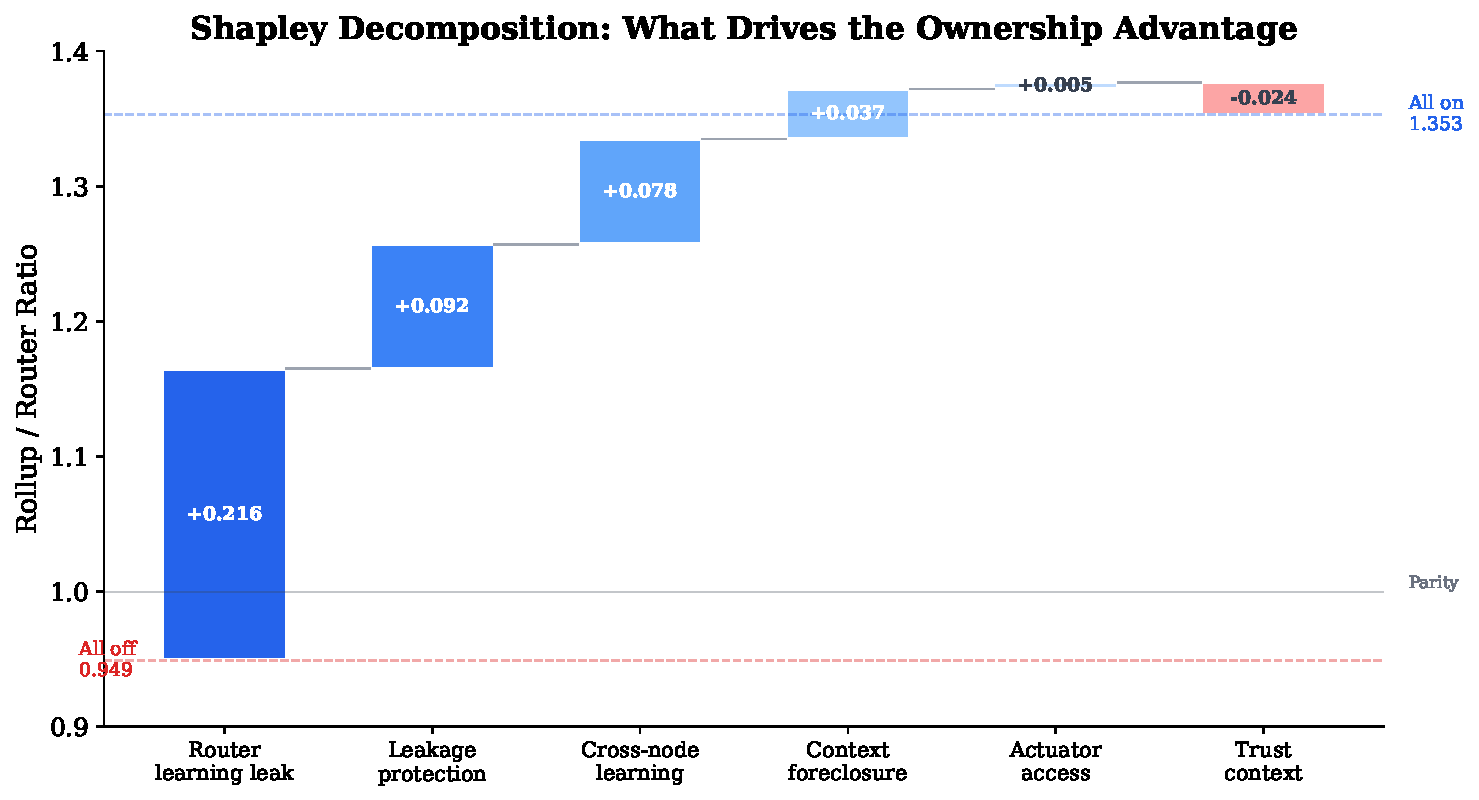
\includegraphics[width=\textwidth]{fig_shapley.pdf}
\caption{Shapley value decomposition of the rollup/router surplus ratio (seed 42; see Table~\ref{tab:shapley} for 5-seed mean $\pm$ std). Router learning leakage is the dominant channel. Note: the foreclosure bar is positive in this seed but negative on average across seeds---see text.}
\label{fig:shapley}
\end{figure}

\subsection{Regime Boundaries}
\label{sec:boundaries}

The baseline is one point in parameter space. Here we trace the boundaries by sweeping each parameter family.

\textbf{Ownership density.} Fixing the owned set at varying fractions (disabling acquisition), the rollup/router ratio increases from below parity at 10\% (where ownership costs exceed the information advantage) to 9.2\% at 90\%. The rollup consistently outperforms the market at all densities because per-interaction channels operate regardless of ownership density.

\textbf{Ownership cost.} The rollup wins at every tested cost level (0.00--0.30 per node per step). At the highest tested overhead (0.30), the rollup still maintains a 26\% net advantage. The dominant channel (router learning leakage) is a cost the router bears regardless of rollup ownership costs.

\textbf{Router learning leakage ($\lambda_R$).} This is the paper's core empirical question, not a settled parameter. $\lambda_R$ governs how aggressively platforms extract and redistribute client operational intelligence---and the entire quantitative story flows downstream from it. We do not claim to know the true value. We claim that the \textit{ranking} of institutional forms is robust across all tested values, while the \textit{magnitude} is an empirical question that specific industries must answer. Table~\ref{tab:lr_sensitivity} presents the full sensitivity:

\begin{table}[H]
\centering
\caption{Rollup/Router ratio vs.\ router learning leakage rate $\lambda_R$ (5 seeds each). This is the most important table in the paper: it shows where the thesis is strong, where it thins, and where it reduces to a slim structural margin.}
\label{tab:lr_sensitivity}
\begin{tabular}{rrr}
\toprule
$\lambda_R$ & Mean ratio & Interpretation \\
\midrule
0.00 & 1.035 & No learning leakage: rollup barely wins \\
0.05 & 1.110 & Mild leakage \\
0.10 & 1.167 & Moderate leakage \\
0.15 & 1.274 & Baseline \\
0.20 & 1.371 & Strong leakage \\
0.30 & 1.615 & Very strong leakage \\
\bottomrule
\end{tabular}
\end{table}

\noindent At $\lambda_R = 0$, the rollup still wins (ratio 1.035) through leakage protection and cross-node learning alone, but the advantage is slim enough that modest agency costs could reverse it. At $\lambda_R = 0.15$ (baseline), the advantage is 26\%. The framework does not resolve which industries sit where on this axis---that is the empirical question it poses. The observed pattern of enterprise AI clients restricting data use (Harvey in legal, Epic in healthcare) suggests that firms believe $\lambda_R > 0$ in their industries, which is evidence for the thesis but not proof of the specific magnitude.

\textbf{Visibility spread.} The gap between internal visibility ($\nu_{\text{int}} = 0.1$) and router visibility ($\nu_{\text{rtr}} = 0.85$) drives the leakage protection channel. How sensitive is the result to this assumed spread? We sweep both parameters independently (3 seeds each). Varying $\nu_{\text{int}}$ from 0.05 to 0.40 (with $\nu_{\text{rtr}}$ fixed at 0.85) changes the ratio from 1.30 to 1.28---the result is insensitive to the exact internal visibility. Varying $\nu_{\text{rtr}}$ from 0.50 to 1.00 (with $\nu_{\text{int}}$ fixed at 0.10) changes the ratio from 1.20 to 1.33---the router's visibility level matters more, as expected. Even at the most favorable visibility for the router ($\nu_{\text{rtr}} = 0.50$, $\nu_{\text{int}} = 0.40$, spread of 0.10), the rollup still wins by $\sim$20\%, because router learning leakage and cross-node learning operate independently of the visibility spread.

\subsection{Data-Isolated Router}
\label{sec:isolated}

The data-isolated router tests the platform's best response: what if the router contractually prevents cross-client data use, eliminating the dominant Shapley channel? The isolated router has the same visibility and interaction parameters as the standard router but charges a per-node subscription fee ($c_{\text{sub}}$ per node per step) instead of extracting learning leakage.

In the baseline, the isolated router generates net surplus of 1,646---13\% above the standard router (1,455) but 12\% below the rollup (1,860). A subscription cost sweep reveals the crossover: the isolated router beats the standard router at every tested subscription cost up to $c_{\text{sub}} = 0.15$ per node per step, where the two converge. Beyond this, the subscription fee outweighs the benefit of data isolation.

The isolated router's leakage cost (0.426 per event) is \textit{lower than the market's} (0.500), because the market exposes interactions at full visibility ($\nu = 1.0$) while the isolated router shields them ($\nu = 0.85$). The ranking market $>$ isolated router for leakage cost means that the isolated router is a genuinely better platform design---but it cannot match the rollup because the rollup also benefits from cross-node learning ($+0.071$ Shapley) and leakage protection ($+0.051$ Shapley) that no platform arrangement can replicate.

This result has a practical implication: firms like Harvey AI that contractually restrict data use are implementing the isolated router. They outperform standard SaaS platforms---but they cannot replicate the ownership advantage. The gap between the isolated router and the rollup represents the irreducible value of common ownership.

\subsection{Superlinearity Without Complementarity}
\label{sec:superlinearity}

With the complementarity coefficient set to zero (the $\kappa_{ij}$ term in Eq.~\ref{eq:match} contributes nothing), the baseline produces a superlinearity ratio of 2.07 (single-seed, seed 42): the combined portfolio generates 107\% more surplus than the sum of its halves. This number requires careful interpretation. The test splits the rollup's 12 owned nodes into two groups of 6 and measures surplus from within-group coordination. Most of the effect is a \textit{network-size} property: the combined portfolio includes 36 cross-group coordination pairs that are excluded from both halves when measured separately. Any network where value comes from connections between nodes would show a similar ratio---this component is not ownership-specific.

The ownership-specific component is layered on top: those 36 cross-group pairs get internal visibility ($\nu = 0.1$) instead of market visibility, so each new coordination opportunity created by combining the groups is also a \textit{higher-quality} opportunity than it would be under separate ownership. Cross-node learning further enhances the combined portfolio's policy quality through greater vertical diversity. The conglomerate premium is real, but the headline ratio overstates the ownership-specific contribution. The more precise claim: each additional node creates new coordination opportunities with every existing node, and common ownership makes those opportunities more valuable per interaction than they would be in the market.

\subsection{Competing Dynamics}
\label{sec:competing}

The parallel-world design cleanly attributes performance differences to institutional form. But it systematically understates the rollup's advantage because it does not model competitive dynamics. In the competing-world simulation, all four forms coexist in a single economy: the rollup starts with 3 nodes, the remaining 27 are split equally among router clients, isolated router clients, and market participants (9 each). Each acquisition \textit{actually removes} the node from its prior regime.

\begin{table}[H]
\centering
\caption{Competing-World Results (50 steps, 30 nodes, passive router, seed 42)}
\label{tab:competing}
\begin{tabular}{lrrrrrr}
\toprule
Regime & Gross & Own.\ cost & Sub.\ cost & Net & Events & Nodes (final) \\
\midrule
Market & 200 & 0 & 0 & 200 & 103 & 9 \\
Router & 283 & 0 & 0 & 283 & 130 & 4 \\
Iso.\ Router & 257 & 0 & 11 & 246 & 149 & 5 \\
Rollup & 495 & 75 & 0 & 420 & 148 & 12 \\
\bottomrule
\end{tabular}
\end{table}

The rollup's net surplus ($420$) exceeds the router's ($283$) by 48\%, the isolated router's ($246$) by 71\%, and the market's ($200$) by $2.1\times$. The rollup acquires 12 of 30 nodes. Across 10 seeds, the rollup wins in all 10 with mean surplus $385$ vs.\ the router's $202$.

\textbf{Router response strategies.} The passive-router assumption is the simplest case. We test two progressively stronger responses, each applied \textit{preemptively from step 0} (not reactively after losing clients) across 10 seeds:

\begin{itemize}[leftmargin=*]
\item \textbf{Preemptive data isolation}: the router eliminates learning leakage ($\lambda_R = 0$) from the first step, becoming a de facto isolated router before losing any clients. This is the router's best response on the dominant Shapley channel. Result: mean rollup surplus $385$, router $202$---the router improves marginally over passive ($202$) but the rollup still wins 10/10. Eliminating the dominant channel preemptively does not overcome the remaining ownership-contingent channels.

\item \textbf{Full defensive}: the router eliminates learning leakage \textit{and} doubles trust investment from step 0---the strongest combination of the router's two available levers. Result: mean rollup surplus $385$, router $202$---virtually identical to isolation alone. Doubling trust investment on top of data isolation adds almost nothing, confirming that trust is the wrong channel (Shapley $-0.011$).
\end{itemize}

\noindent The key result is not that the rollup wins three times, but \textit{what the strategies reveal about the mechanism}. The router's strongest available move---preemptive data isolation, addressing the dominant channel before any competitive damage---narrows the gap from 1.91$\times$ to 1.90$\times$. The residual advantage is entirely from ownership-contingent channels (cross-node learning, internal visibility) that no platform strategy can address, because they require owning the nodes, not just serving them differently.

The parallel and competing results reinforce each other. The parallel model identifies \textit{which channels} create the structural edge. The competing model shows what happens when that edge compounds: not a permanent marginal advantage, but a tipping dynamic that shifts the economy toward ownership.

\subsection{Industry Predictions}
\label{sec:industries}

The framework maps industries to positions in parameter space via three dimensions: \textit{durability} (how long revealed context remains exploitable, governed by $\rho_L$), \textit{specificity} (how much competitive value each revelation destroys, governed by leakage sensitivity bounds), and \textit{transferability} (how much operational knowledge transfers across nodes, governed by $\tau$). We calibrate all 35 services verticals from \citet{sequoia2025services}, who classify AI-native services along intelligence-vs-judgement and outsourced-vs-insourced axes. Our parameter mapping is: intelligence ratio $\to$ transferability ($\tau$), context sensitivity $\to$ specificity ($\ell$), and competitive half-life $\to$ durability ($\rho_L$). Table~\ref{tab:industries} reports the full results, grouped by the Sequoia quadrant.

\begin{table}[p]
\centering
\caption{Services Taxonomy: Predicted Rollup Advantage by Industry (3-seed mean $\pm$ std). Industries from \citet{sequoia2025services}, grouped by quadrant. D$\times$S$\times$T = durability $\times$ specificity $\times$ transferability (H/M/L). Shading intensity reflects advantage magnitude.}
\label{tab:industries}
\vspace{-4pt}
{\footnotesize
\renewcommand{\arraystretch}{0.92}
\begin{tabular}{llclr}
\toprule
Industry & TAM & D$\times$S$\times$T & Quadrant & Rollup/Router \\
\midrule
Cybersecurity & \$30B+ & H$\times$H$\times$M & Watch & \cellcolor{green!28} $1.276 \pm .044$ \\
Pharmacy back-office & \$30B+ & M$\times$M$\times$H & Next wave & \cellcolor{green!24} $1.263 \pm .039$ \\
KYC / AML & \$30--50B & H$\times$H$\times$M & Autopilot & \cellcolor{green!22} $1.258 \pm .041$ \\
Claims adjusting & \$50--80B & M$\times$M$\times$H & Autopilot & \cellcolor{green!21} $1.255 \pm .039$ \\
Mortgage origination & \$30--50B & M$\times$M$\times$H & Autopilot & \cellcolor{green!21} $1.255 \pm .039$ \\
Medical admin & \$20B+ & M$\times$M$\times$H & Next wave & \cellcolor{green!21} $1.255 \pm .039$ \\
Supply chain \& procurement & \$200B+ & H$\times$H$\times$M & Next wave & \cellcolor{green!21} $1.254 \pm .041$ \\
Accounting \& audit & \$50--80B & H$\times$H$\times$M & Autopilot & \cellcolor{green!20} $1.251 \pm .042$ \\
Clinical trials / CRO & \$80B+ & H$\times$H$\times$M & Watch & \cellcolor{green!20} $1.251 \pm .042$ \\
ERP implementation & \$50B+ & H$\times$H$\times$M & Watch & \cellcolor{green!20} $1.251 \pm .040$ \\
Freight brokerage & \$100B+ & L$\times$M$\times$H & Watch & \cellcolor{green!19} $1.248 \pm .040$ \\
Insurance brokerage & \$140--200B & M$\times$M$\times$H & Autopilot & \cellcolor{green!18} $1.247 \pm .040$ \\
Real estate closing & \$20--25B & M$\times$M$\times$H & Autopilot & \cellcolor{green!18} $1.245 \pm .040$ \\
SEO / SEM & \$50B+ & L$\times$M$\times$H & Watch & \cellcolor{green!18} $1.245 \pm .040$ \\
Recruitment \& staffing & \$200B+ & M$\times$M$\times$H & Watch & \cellcolor{green!18} $1.245 \pm .040$ \\
Cost estimation & \$16B & M$\times$M$\times$M & Autopilot & \cellcolor{green!17} $1.244 \pm .038$ \\
Market research & \$45B & M$\times$M$\times$M & Watch & \cellcolor{green!17} $1.244 \pm .038$ \\
Tax advisory & \$30--35B & H$\times$H$\times$L & Autopilot & \cellcolor{green!17} $1.242 \pm .044$ \\
Healthcare rev cycle & \$50--80B & M$\times$L$\times$H & Autopilot & \cellcolor{green!17} $1.241 \pm .040$ \\
Payroll \& compliance & \$50--70B & M$\times$L$\times$H & Autopilot & \cellcolor{green!16} $1.238 \pm .039$ \\
Architecture & \$25B+ & M$\times$M$\times$M & Watch & \cellcolor{green!15} $1.237 \pm .039$ \\
Paralegal / LPO & \$36B & H$\times$H$\times$L & Autopilot & \cellcolor{green!15} $1.236 \pm .042$ \\
PR \& comms & \$20B+ & M$\times$M$\times$M & Copilot & \cellcolor{green!15} $1.235 \pm .038$ \\
Management consulting & \$300B+ & H$\times$H$\times$L & Copilot & \cellcolor{green!14} $1.234 \pm .043$ \\
Wealth mgmt ops & \$30B+ & H$\times$H$\times$L & Next wave & \cellcolor{green!14} $1.234 \pm .043$ \\
Advertising & \$100B+ & L$\times$M$\times$H & Watch & \cellcolor{green!14} $1.233 \pm .039$ \\
Fund administration & \$15--20B & H$\times$H$\times$L & Next wave & \cellcolor{green!14} $1.233 \pm .043$ \\
Legal, transactional & \$20--25B & H$\times$H$\times$L & Autopilot & \cellcolor{green!12} $1.228 \pm .037$ \\
Executive search & \$20B+ & H$\times$H$\times$L & Copilot & \cellcolor{green!12} $1.228 \pm .042$ \\
Patent / IP & \$15--20B & H$\times$H$\times$L & Watch & \cellcolor{green!12} $1.228 \pm .037$ \\
Graphic / UX design & \$30B+ & L$\times$L$\times$H & Copilot & \cellcolor{green!11} $1.223 \pm .039$ \\
IT managed services & \$100B+ & L$\times$L$\times$H & Autopilot & \cellcolor{green!9} $1.219 \pm .039$ \\
Corporate training & \$50B+ & L$\times$L$\times$H & Watch & \cellcolor{green!9} $1.219 \pm .039$ \\
Admin assistants & \$80B+ & L$\times$L$\times$H & Watch & \cellcolor{green!8} $1.215 \pm .038$ \\
Travel management & \$15B+ & L$\times$L$\times$H & Watch & \cellcolor{green!8} $1.215 \pm .038$ \\
\bottomrule
\end{tabular}
}
\end{table}

Three patterns emerge. First, the rollup dominates in \textit{every} tested vertical---the advantage ranges from 21.5\% (travel, admin) to 27.6\% (cybersecurity). The mechanism is universal; only the magnitude is industry-specific.

Second, the advantage is driven by the \textit{interaction} of durability and transferability, not by either dimension alone. The highest-scoring industry is cybersecurity (1.28$\times$)---not because it has the most durable context (legal and patent/IP have higher $\rho_L$), but because it combines high durability with moderate transferability. A zero-day discovered at one portfolio company protects all others; an incident response playbook developed for one client improves response across the portfolio. Pure durability without transferability (legal transactional, patent/IP: 1.23$\times$) scores lower because cross-node learning---the second-largest Shapley channel---is weak when each engagement is too bespoke for operational patterns to transfer across nodes. The bottom of the table---travel, admin, IT services (1.22$\times$)---consists of verticals where context expires quickly and carries little competitive value.

Third, the Sequoia taxonomy's ``autopilot territory'' and our framework's highest-advantage industries overlap substantially but are not identical, because our model captures the durability$\times$transferability interaction independently of the intelligence-vs-judgement axis. Cybersecurity appears in the ``watch'' quadrant but scores highest in our framework. IT managed services is the most automatable autopilot vertical but scores lowest, because its context is ephemeral and non-specific.

\textbf{These are testable predictions.} The framework predicts that AI-driven consolidation should appear earliest in high-$\rho_L$, high-$\ell$ verticals and be weakest in low-$\rho_L$, low-$\ell$ verticals. The $\lambda_R$ boundary condition adds a further prediction: in verticals where platforms can credibly commit to data isolation ($\lambda_R \to 0$), the rollup advantage narrows to $\sim$3.5\%. Enterprise AI providers offering strict data isolation (Harvey in legal) are implementing the isolated router---addressing the dominant channel but unable to replicate the cross-node learning and internal visibility that ownership provides.

%=============================================================================
\section{Discussion}
%=============================================================================

\subsection{Reinterpreting the Coasean Singularity}

The Coasean singularity thesis---that AI-driven transaction cost reduction will dissolve firms into agent-mediated markets---captures one real channel while missing two others. Yes, AI reduces the cost of market coordination. But simultaneously, platform intermediation may \textit{amplify} information leakage (the dominant channel in our Shapley decomposition), and ownership enables cross-node learning that market coordination cannot replicate. The net effect on firm boundaries depends on the magnitude of these countervailing forces.

Our results suggest a conditional revision of the Coasean singularity thesis. The standard account assumes that platform intermediation reduces information frictions. We model the hypothesis that intermediation can \textit{amplify} leakage---when a platform ingests client operational data to improve its service, that improvement benefits the client's competitors. If this hypothesis holds (and real-world practices like Harvey AI's data restrictions suggest firms believe it does), it is the dominant channel driving ownership advantage, producing $1.9\times$ the leakage cost of the open market in our simulation ($0.93$ vs.\ $0.50$ per event). The data-isolated router---a platform that contractually prevents this---recovers most of the gap but cannot match the rollup, because ownership captures channels (cross-node learning, internal visibility) that no contractual arrangement can replicate.

The updated Coasean logic: \textit{in AI-intensive industries with local, leakage-sensitive context, intermediation may not reduce information frictions but amplify them.} Every interaction through a SaaS platform trains the platform's model, and that model serves your competitors. Ownership avoids this entirely. The firm exists not to reduce transaction costs but to prevent the extraction and redistribution of its scarce context. The firm does not just persist; it expands because each acquisition marginally improves its information position relative to competitors. This is the cybernetic arbitrage: the spread between the market's valuation of assets as isolated operations and their actual value as nodes in an AI-coordinated portfolio---a spread that is small per-node but cumulative across the vertical.

\subsection{Autopilots Are Routers}

A growing thesis in venture capital holds that AI-native services companies---``autopilots'' that sell the \textit{work} rather than the \textit{tool}---will capture the \$6 of services spend for every \$1 of software spend \citep{sequoia2025services}. The argument: every improvement in the underlying model makes the autopilot faster and cheaper, compounding a data advantage from doing the work at scale. Autopilots are projected to dominate outsourced, intelligence-heavy verticals first (insurance brokerage, healthcare billing, tax compliance) and expand toward judgement-heavy work as AI matures.

Our framework reveals a structural tension in this thesis. \textbf{The autopilot is a more capable router, but a router nonetheless.} When Harvey drafts an NDA, it intermediates the coordination between client and counterparty. When Anterior processes a prior authorization, it intermediates between provider and payer. The autopilot \textit{does} the work, but it does not \textit{own} the node where context is born. It sees the client's operational data---exception patterns, pricing sensitivity, negotiation positions---and this creates the same information economics our model formalizes:

\begin{itemize}[leftmargin=*]
\item If the autopilot uses client data to improve its service for \textit{all} clients, it is a standard router with learning leakage. Each client's operational intelligence is ingested, systematized, and deployed to serve competitors.

\item If the autopilot commits to data isolation (per-client model weights, contractual data restrictions), it is our isolated router: better than the standard platform, but unable to capture the cross-node learning and internal visibility channels that ownership provides.
\end{itemize}

\noindent The driving effect is strategic: the context owner knows that revealing information to an external party is costly, so they rationally withhold. When a law firm hires Harvey to draft an NDA, sharing its full negotiation strategy would produce a better draft---but it also exposes that strategy to an entity the firm does not control. The firm faces the revelation-leakage tradeoff and, in our simulation, chooses partial revelation in $\sim$20\% of such interactions. Worse drafts, worse coordination, less surplus. When the rollup's own subsidiary drafts the NDA, the firm faces no such tradeoff: internal visibility is low ($\nu = 0.1$), so full revelation is cheap, and the rollup reveals freely in 88\% of events. The ownership advantage is not that the rollup has better technology---it is that firms are willing to reveal more to an entity they own than to one they hire.

The prediction is not that autopilots will fail---they will likely outperform copilots and general SaaS platforms, exactly as \citet{sequoia2025services} argues. The prediction is that autopilots face the same structural ceiling as any intermediary: they can eliminate the learning leakage channel through data isolation, but they cannot replicate the cross-node learning, internal visibility, and competitive foreclosure that ownership provides. In verticals where these channels matter (legal, tax, accounting, cybersecurity---the top of Table~\ref{tab:industries}), the endgame is not the autopilot but the entity that owns the firms the autopilot serves. The autopilot is the wedge; the rollup is the moat.

\subsection{Where the Framework Predicts Rollup Dominance---and Where It Does Not}

The regime map (Section~\ref{sec:regimemap}) and industry calibrations (Section~\ref{sec:industries}) generate testable predictions about where different institutional forms should dominate:

\begin{enumerate}[leftmargin=*]
\item \textbf{The rollup wins where context is durable and specific} ($\rho_L > 0.7$, high $\ell$). Legal transactional work, tax advisory, and specialized financial services occupy this region. These verticals should see AI-driven consolidation first.

\item \textbf{The data-isolated router wins where platforms can credibly commit to isolation}. When $\lambda_R \to 0$ (through contractual restriction or technical architecture), the rollup advantage narrows to $\sim$3.5\%. If ownership costs are also high (agency costs, regulatory overhead), the isolated router can dominate. This predicts that platforms committing to data isolation---contractually guaranteeing that one client's operational data will not be used to serve another---should outperform platforms that pool client data across their user base.

\item \textbf{The router/market wins where context is short-lived and non-specific} ($\rho_L < 0.3$, low $\ell$). IT managed services, commodity logistics, and contexts where information is too ephemeral to exploit. Here, leakage protection contributes little, and the platform's breadth advantage in learning from standardized, transferable patterns may offset the rollup's ownership channels.

\item \textbf{The rollup thesis fails when cross-node learning is absent}. If operations are too heterogeneous for knowledge to transfer across portfolio companies ($\tau \to 0$), or if AI cannot extract transferable patterns, the second-largest channel disappears. Combined with data isolation ($\lambda_R = 0$), this leaves only leakage protection---a $\sim$5\% advantage that may not justify ownership overhead.
\end{enumerate}

\noindent The framework does not predict a universal answer. It maps parameter space to institutional form dominance, generating industry-specific predictions that can be tested against observed patterns of AI-era consolidation.

\subsection{Implications for Industrial Organization}

Three implications follow from the framework that are worth stating explicitly.

\textbf{Cross-node learning has increasing returns.} The transfer bonus in the model scales with the number of distinct verticals in the owned portfolio ($\tau \cdot |\{v_k\}| / K$). This creates a positive feedback loop: more nodes owned $\to$ more verticals covered $\to$ richer cross-node learning $\to$ higher acquisition value of the next node $\to$ more nodes owned. The first entity to reach critical mass in a vertical has a compounding advantage that late entrants cannot overcome, because they face a cold-start problem: they cannot match the cross-node learning without the nodes, and they cannot justify acquiring the nodes without the learning. This implies that AI-era consolidation, once it begins in a vertical, should exhibit winner-take-most dynamics---not because of demand-side network effects (as in platform markets) but because of supply-side learning economies that are structurally ownership-contingent.

\textbf{Operational access can approximate ownership for information flows.} The model treats ownership as binary: a node is owned or it is not. In practice, deep operational engagement---consulting, advisory, integration work---can provide signal quality approaching ownership levels without requiring financial acquisition. A firm embedded inside a company for twelve weeks, observing workflows and exception handling at full depth, achieves something close to the rollup's internal visibility ($\sigma_{\text{own}} = 0.9$) without taking an equity position. This suggests the rollup's information advantage can be partially achieved through services relationships, with financial acquisition reserved for nodes where the context is durable enough to justify the ownership overhead. The consulting engagement becomes the sensing layer; the acquisition follows only where the learning compounds.

\textbf{The parameter space determines whether platforms evolve toward ownership.} The framework predicts not just which regime dominates, but whether the platform-to-ownership transition occurs at all. Where context is durable and specific (high $\rho_L$, high $\ell$---legal, tax, cybersecurity), the leakage cost per unit is high enough that rational actors withhold from intermediaries, degrading the platform's data quality and pushing it toward ownership as the only reliable path to full context access. The historical analogue is Metropolis, a parking technology company that could not sell its software to parking garage operators and instead acquired the garages themselves.

But where context is ephemeral and non-specific (low $\rho_L$, low $\ell$---advertising, logistics, commodity transactions), the platform model can be stable \textit{even with full learning leakage}. Meta's advertising platform extracts retailer conversion data through installed tracking pixels and uses it to optimize ad delivery for all advertisers, including each retailer's competitors. Retailers accept this because the data is high-volume but low-value-per-unit: no individual retailer's conversion events constitute a durable competitive asset, and the value of Meta's ad optimization exceeds the leakage cost. This is the standard router in our model---but operating in the region of parameter space where the rollup advantage is smallest ($\sim$1.22$\times$) and the leakage cost is low enough that clients rationally participate.

The implication is that the autopilot-to-ownership transition is industry-dependent. In the top of Table~\ref{tab:industries}, it is the likely equilibrium: the autopilot is the wedge, but ownership is the moat. In the bottom, the platform model persists because there is not enough durable, specific context to justify the overhead of ownership---and not enough leakage cost to drive clients away.

\textbf{Model training as a new form of cross-node learning.} As AI labs seek operational data for model improvement---through instrumentation partnerships, screen observation, and workflow capture---a question arises: does the model itself absorb the cross-node learning channel? If a lab has trained on 10,000 dental practices across 50 portfolios, the model already knows the optimal scheduling approach. The rollup's ability to observe its own five practices and transfer learnings adds nothing the model does not already provide. In this view, cross-node learning ($\sim$23\% of the Shapley effect) is partially commoditized by model training: the ``what works at dental practices'' knowledge becomes embedded in the model and available to everyone, not just the owner.

The rollup's remaining advantage shifts from \textit{learning what works} (which the model increasingly provides) to \textit{knowing what is happening right now and having the authority to act on it}. The model knows general patterns from historical training data. The rollup knows that this specific practice's lead hygienist quit yesterday, that the local competitor just closed, that the insurance contract is up for renegotiation next month. These are real-time, firm-specific observations that training pipelines cannot capture at the same latency---and that require ownership-level visibility ($\nu = 0.1$) to observe at all. The rollup's advantage migrates from pattern recognition to operational latency and actuator access.

The emerging structure of lab-PE partnerships is consistent with this analysis. Labs are pursuing joint ventures with portfolio owners rather than commercial API relationships---seeking ownership-equivalent context access through equity alignment. This implicitly validates the framework's prediction: commercial access does not provide the context depth that ownership does, and the labs are reaching for ownership-like structures to close the gap.

\subsection{Limitations}

Several limitations warrant discussion.

First, and most critically, while we model ownership costs (overhead and integration friction), we do not model \textit{agency costs}---and agency costs may be the binding constraint on the rollup thesis. In practice, each subsidiary's management has its own incentives---empire-building, risk aversion, headcount padding, pet projects---that diverge from the parent company's goal of maximizing portfolio value. The more subsidiaries owned, the harder each is to monitor, and the more value leaks to misaligned behavior. \citet{berger1995} found that diversified firms trade at a 13--15\% discount to the sum of their parts, and \citet{jensen1986} attributes this largely to inefficient internal capital allocation driven by managerial self-interest. Our flat ownership cost ($c_{\text{overhead}}$ per node per step) understates this problem: real agency costs are likely \textit{convex} in portfolio size, because each additional subsidiary dilutes management attention and introduces cross-subsidiary politics. At the baseline rollup advantage of $\sim$26\%, convex agency costs could plausibly eliminate the margin.

The deeper issue is that context access and context \textit{compounding} are not the same thing. A large consulting firm like BCG or McKinsey has had deep operational access to thousands of companies over decades---arguably more ``context born at the node'' than any rollup could accumulate. Yet this context does not compound: it lives in slide decks, in partners' heads, in institutional memory that walks out the door with departing staff. The organizational structure of a consulting firm---partner incentives misaligned with firm-wide knowledge management, practice areas operating semi-independently, no central system of record for operational observations---is itself an agency cost that prevents the conversion of contact into structured, reusable intelligence. Our model assumes that the rollup can convert ownership into a central, compounding intelligence layer. Whether this assumption holds depends on whether AI-enabled coordination can reduce the organizational overhead of multi-node management sufficiently to overcome the agency costs that have historically made conglomerates value-destructive. This is the strongest version of the counterargument to our thesis, and the model does not resolve it.

Second, the model uses a scalar policy quality rather than heterogeneous policies across nodes. In practice, the value of cross-node learning depends on the transferability of operational knowledge, which varies across industries and firm types.

Third, the parallel-world structural advantage is scale-invariant: at 200 nodes with 10 verticals (50 seeds, mean ratio 1.23, 50/50 pass) and 1000 nodes with 20 verticals (ratio 1.22), the mechanisms produce consistent results. Verticals scale proportionally with graph size ($\sim$1 vertical per 20 nodes) to maintain comparable industry structure. The competing-world tipping dynamic also scales, but requires sufficient simulation duration for the rollup to accumulate critical ownership density. At 200 nodes with the default acquisition rate (one node per 5 steps), a 100-step simulation reaches only $\sim$15\% density---too short for tipping. Extending to 500 steps (5 seeds), the rollup reaches 55\% density, the router collapses to 8--12 nodes (out of 200), and the surplus ratio reaches 1.45--1.60. The tipping dynamic is not scale-dependent; it simply requires enough time to accumulate ownership.

Fourth, the model does not capture \textit{strategic information withholding} by router clients. In practice, firms aware of router learning leakage contractually restrict data use: enterprise AI providers like Harvey (legal AI) face strict limitations on using client data to train models that serve other clients. This withholding is rational---it reduces the leakage cost---but it also reduces the value the platform can deliver, creating a tension between service quality and competitive exposure. In our simulation, the revelation optimizer always chooses maximum revelation because match quality gains dominate; a model with stronger leakage costs or contractual restrictions could produce endogenous withholding, further degrading the router's value proposition.

Fifth, the model treats ownership as a per-node property: each owned node gets lower visibility, higher actuator authority, and trust investment, regardless of how many other nodes in the same vertical are also owned. It does not capture \textit{vertical completion effects}---the additional value that accrues when a rollup owns every firm in a sector, including the elimination of within-sector competitive leakage, monopoly pricing power, and complete information over all sector activity.

%=============================================================================
\section{Conclusion}
%=============================================================================

This paper develops a framework that maps the parameter space of information economics to institutional form dominance, comparing four forms---fragmented markets, platform routers, data-isolated routers, and cybernetic rollups---over a directed graph economy. The framework identifies three mechanisms driving ownership advantage (router learning leakage, cross-node learning, leakage protection), establishes their ranking as stable across calibrations, and generates testable predictions about which industries should see AI-driven consolidation.

The central finding is that ownership advantage is robust but not universal. The rollup dominates in verticals where context is durable and specific---legal transactional work, tax advisory, specialized financial services. The advantage narrows where context is short-lived (IT managed services: 1.22$\times$) and nearly vanishes where platforms can credibly commit to data isolation and cross-node learning is absent. A data-isolated router---the platform's best response---eliminates the dominant channel but cannot replicate the cross-node learning and internal visibility that ownership provides, trailing the rollup by $\sim$12\% at baseline calibration.

For theory, the contribution is the framework itself: a mapping from parameter space to institutional form dominance that identifies which mechanisms matter, in what order, and under what conditions. For practice, it generates predictions: AI-driven consolidation should appear earliest in high-durability, high-specificity verticals (legal, tax, specialized finance); platform providers should invest in credible data isolation; and firms using SaaS platforms for operationally sensitive coordination should understand that each interaction may train a model that serves their competitors.

The cybernetic arbitrage is the spread between the market's valuation of assets as isolated operations and their actual value as nodes in an AI-coordinated portfolio where context is internalized rather than leaked. Where that spread exists---and this paper maps where it should---ownership captures the value that AI creates.

%=============================================================================
% Bibliography
%=============================================================================

\bibliographystyle{aer}

\begin{thebibliography}{99}

\bibitem[Agrawal et~al.(2018)]{agrawal2018}
Agrawal, Ajay, Joshua Gans, and Avi Goldfarb. 2018. ``Prediction Machines: The Simple Economics of Artificial Intelligence.'' \textit{Harvard Business Review Press}.

\bibitem[Armstrong(2006)]{armstrong2006}
Armstrong, Mark. 2006. ``Competition in Two-Sided Markets.'' \textit{RAND Journal of Economics} 37(3): 668--691.

\bibitem[Benzell and Brynjolfsson(2024)]{benzell2024}
Benzell, Seth G., and Erik Brynjolfsson. 2024. ``AI and the Boundary of the Firm.'' Working paper.

\bibitem[Bonatti et~al.(2022)]{bonatti2022}
Bonatti, Alessandro, Munther Dahleh, Thibaut Horel, and Amir Nouripour. 2022. ``Selling Information in Competitive Environments.'' arXiv:2202.08780.

\bibitem[Berger and Ofek(1995)]{berger1995}
Berger, Philip G., and Eli Ofek. 1995. ``Diversification's Effect on Firm Value.'' \textit{Journal of Financial Economics} 37(1): 39--65.

\bibitem[Brynjolfsson and Mitchell(2017)]{brynjolfsson2017}
Brynjolfsson, Erik, and Tom Mitchell. 2017. ``What Can Machine Learning Do? Workforce Implications.'' \textit{Science} 358(6370): 1530--1534.

\bibitem[Christensen(1997)]{christensen1997}
Christensen, Clayton M. 1997. \textit{The Innovator's Dilemma}. Boston: Harvard Business School Press.

\bibitem[Chopra et~al.(2024)]{chopra2024}
Chopra, Ayush, et~al. 2024. ``What Can We Learn from a Billion Agents?'' arXiv:2501.10025.

\bibitem[Coase(1937)]{coase1937}
Coase, Ronald H. 1937. ``The Nature of the Firm.'' \textit{Economica} 4(16): 386--405.

\bibitem[Danco(2017)]{danco2017}
Danco, Alex. 2017. ``Understanding Abundance.'' \textit{Social Capital}, February.

\bibitem[Grossman and Hart(1986)]{grossman1986}
Grossman, Sanford J., and Oliver D. Hart. 1986. ``The Costs and Benefits of Ownership: A Theory of Vertical and Lateral Integration.'' \textit{Journal of Political Economy} 94(4): 691--719.

\bibitem[Hart and Moore(1990)]{hart1990}
Hart, Oliver, and John Moore. 1990. ``Property Rights and the Nature of the Firm.'' \textit{Journal of Political Economy} 98(6): 1119--1158.

\bibitem[Hart(1995)]{hart1995}
Hart, Oliver. 1995. \textit{Firms, Contracts, and Financial Structure}. Oxford: Clarendon Press.

\bibitem[Hobart(2024)]{hobart2024routers}
Hobart, Byrne. 2024. ``Routers, Apps, AGI.'' \textit{The Diff}, October.

\bibitem[Jensen(1986)]{jensen1986}
Jensen, Michael C. 1986. ``Agency Costs of Free Cash Flow, Corporate Finance, and Takeovers.'' \textit{American Economic Review} 76(2): 323--329.

\bibitem[Lang and Stulz(1994)]{lang1994}
Lang, Larry H.P., and Ren\'{e} M. Stulz. 1994. ``Tobin's q, Corporate Diversification, and Firm Performance.'' \textit{Journal of Political Economy} 102(6): 1248--1280.

\bibitem[Larson(2025)]{larson2025cybernetic}
Larson, Soren. 2025. ``Cybernetic Arbitrage: AI is Inverting Aggregation Theory.'' \textit{hypersoren.xyz}, December.

\bibitem[Parker et~al.(2016)]{parker2016}
Parker, Geoffrey G., Marshall W. Van Alstyne, and Sangeet Paul Choudary. 2016. \textit{Platform Revolution}. New York: W.W. Norton.

\bibitem[Azhar(2024)]{azhar2024}
Azhar, Azeem. 2024. ``From ChatGPT to a Billion Agents.'' \textit{Exponential View}, December.

\bibitem[Shapiro(2024)]{shapiro2024}
Shapiro, David. 2024. ``Billions of Agents.'' September.

\bibitem[Toma\v{s}ev et~al.(2025)]{tomasev2025}
Toma\v{s}ev, Nenad, Matija Franklin, Joel Z. Leibo, Julian Jacobs, William A. Cunningham, Iason Gabriel, and Simon Osindero. 2025. ``Virtual Agent Economies.'' arXiv:2509.10147.

\bibitem[Bek(2026)]{sequoia2025services}
Bek, Julien. 2026. ``Services: The New Software.'' \textit{Sequoia Capital}, March.

\bibitem[Shahidi et~al.(2025)]{shahidi2025}
Shahidi, Peyman, Gili Rusak, Benjamin S. Manning, Andrey Fradkin, and John J. Horton. 2025. ``The Coasean Singularity? Demand, Supply, and Market Design with AI Agents.'' NBER Working Paper.

\bibitem[Rochet and Tirole(2003)]{rochet2003}
Rochet, Jean-Charles, and Jean Tirole. 2003. ``Platform Competition in Two-Sided Markets.'' \textit{Journal of the European Economic Association} 1(4): 990--1029.

\bibitem[Williamson(1975)]{williamson1975}
Williamson, Oliver E. 1975. \textit{Markets and Hierarchies: Analysis and Antitrust Implications}. New York: Free Press.

\bibitem[Williamson(1985)]{williamson1985}
Williamson, Oliver E. 1985. \textit{The Economic Institutions of Capitalism}. New York: Free Press.

\end{thebibliography}

\end{document}
